% use paper, or submit
% use 11 pt (preferred), 12 pt, or 10 pt only

%\documentclass[letterpaper, preprint, paper,11pt]{AAS}	% for preprint proceedings
\documentclass[letterpaper, paper,11pt]{AAS}		% for final proceedings (20-page limit)
%\documentclass[letterpaper, paper,12pt]{AAS}		% for final proceedings (20-page limit)
%\documentclass[letterpaper, paper,10pt]{AAS}		% for final proceedings (20-page limit)
%\documentclass[letterpaper, submit]{AAS}			% to submit to JAS

\usepackage{AAS_packages}
%\usepackage{subfigure} % have subcaption in use instead
%\usepackage[notref,notcite]{showkeys}  % use this to temporarily show labels

\PaperNumber{XX-XXX}

\begin{document}

\title{Real Time Adaptive Shape Reconstruction for Asteroid Landing}

\author{Shankar Kulumani and Taeyoung Lee\thanks{Mechanical and Aerospace Engineering, George Washington University, 800 22nd St NW, Washington, DC 20052, Tel: 202-994-8710, Email: \href{mailto:skulumani@gwu.edu}{\{skulumani,tylee\}@gwu.edu}.}
}


\maketitle{} 		

\begin{abstract}
    Knowledge of the shape of an asteroid is crucial for spacecraft operations.
    The standard method of determining the gravitational potential, through the use of a polyhedral potential model, is dependent on the shape model.
    Furthermore, accurate landing or low altitude operations requires an accurate knowledge of the surface topology. 
    The typical approach to shape determination requires an extensive ``mapping'' phase of the mission over which extensive measurements are collected and transmitted for Earth-based processing.
    Instead, we present an efficient method for estimating the shape of an asteroid in real time.
    Range measurements of the surface are used to incrementally correct an initial shape estimate.
    This update procedure occurs in real time and provides a more accurate model of the asteroid shape.
    This shape model is then used in a nonlinear controller to track a desired trajectory about the asteroid.
    The closed loop approach allows a spacecraft to approach and operate near an unknown asteroid while autonomously generating a surface shape model.
    We demonstrate this approach through a dynamic simulation about asteroid 4769 Castalia.
\end{abstract}

\section{Introduction}\label{sec:introduction}
% Motivation for missions/studying asteroids
Small solar system bodies, such as asteroids and comets, continue to remain a focus of scientific study.
The small size of these bodies prevents the formation of large internal pressures and temperatures which help to preserve the early chemistry of the solar system.
This insight offers additional detail into the formation of the Earth and also of the probable formation of other extrasolar planetary bodies.
Of particular interest are those near-Earth asteroids (NEA) which inhabit heliocentric orbits in the vicinity of the Earth. 
These easily accessible bodies provide attractive targets to support space industrialization, mining operations, and scientific missions.
In spite of the significant interest, and the extensive research by the community, the operation of spacecraft near small bodies remains a challenging problem.

% dynamics are difficult around asteroids
The dynamic environment around asteroids is strongly perturbed and challenging for analysis and mission operations~\cite{scheeres2012}.
Due to their low mass, which in turn causes a low gravitational attraction, asteroids may have irregular shapes.
Furthermore, asteroids may also have a chaotic spin state due to the absorption and emittance of solar radiation~\cite{rubincam2000}.
As a result, approaches utilizing an inverse square gravitational model do not capture the  true dynamic environment.
In addition, the vast majority of asteroids are difficult to track and characterize using ground based sensors.
Due to their small size, frequently less than \SI{1}{\kilo\meter}, and low albedo, the reflected energy of these asteroids is insufficient for reliable detection or tracking.
Therefore, the dynamics model of the asteroid is relatively coarse prior to in situ measurements from a dedicated spacecraft.
As a result, any spacecraft mission to an asteroid must include the ability to update the dynamic model given in situ measurements and remain robust to unmodelled forces.

Another key dynamic consideration is the coupling between rotational and translational states around the asteroid.
The coupling is induced due to the different gravitational forces experienced on various portions of the spacecraft. 
The effect of the gravitational coupling is related to the ratio of the spacecraft size and orbital radius~\cite{hughes2004}.
For operations around asteroids, the ratio is relatively large which causes a much larger coupling between the translational and rotational states.
References~\citenum{elmasri2005} and~\citenum{sanyal2004a} investigated the coupling of an elastic dumbbell spacecraft in orbit about a central body, but only considered the case of a spherically symmetric central body.
Furthermore, the spacecraft model is assumed to remain in a planar orbit.
As a result, these developments are not directly applicable to motion about an asteroid, which experiences highly non-Keplerian motion.
Reference~\citenum{misra2015b} investigated the effect of coupled motion on long term trajectories around asteroids.
However, the analysis only considered a second order spherical harmonic gravitational potential model. 
Therefore, these results are only valid when far from the asteroid surface and will diverge when used within the Brillouin sphere.

% Gravity model is important and dependent on shape
An accurate gravitational potential model is critical for performing low altitude and/or surface operations around asteroids.
Due to the irregular shape, trajectories will pass within the Brillouin sphere, where the typical spherical harmonic model diverges from the true gravitational potential.
The standard approach for asteroid missions is to compute the gravitational potential using a polyhedron potential model~\cite{werner1996}.
The polyhedral potential model provides the exact gravitational potential, and subsequently the gravitational acceleration, for a given triangular faceted shape model of an asteroid.
The method provides the exact potential at any point outside the body for a given shape model.
As a result, the accuracy of the gravitational potential is primarily dependent on the accuracy with which the shape model represents the true surface.
A high fidelity shape, which necessarily has many vertices and faces, is required for an accurate computation of the gravitational acceleration and enabling low altitude operations.

% Challenges involved in operation near asteroids (gravity, shape, distance)
% generating the shape from the ground is difficult
Prior to the arrival of a spacecraft at an asteroid, Earth based sensors are used to characterize the body.
Using both optical and radar sensors allows for the precise orbit of the asteroid to be determined.
Another vital task is the determination of the asteroid shape from radar data~\cite{hudson1994,busch2011}.
This is a challenging problem as it requires the simultaneous estimation of the asteroid spin state and shape.
Furthermore, determining the shape from radar is currently the only Earth-based technique that can produce detailed three-dimensional shape information of near-Earth objects~\cite{greenberg2015}.
The current approach is based on an estimation scheme which iteratively perturbs a shape to match given radar data.
This computationally intensive approach is only able to capture the gross size and shape and is unable to capture the small surface features of the asteroid.
Frequently, only a coarse model is possible from the ground and an accurate shape must be determined only after a spacecraft has rendezvoused with the asteroid.
As a result, upon arrival the gravitational environment near the asteroid is poorly modeled as the shape of the asteroid is not accurate.
Therefore, the polyhedron potential model is not appropriate immediately upon arrival but rather only after the shape has been determined.

% on arrival spacecraft spend long periods mapping, and depending on mission this might be unallocable
On approach to an asteroid, spacecraft navigation and guidance is primarily based on ground measurements.
After arrival, a spacecraft will generally spend months or years in a mapping mission phase~\cite{kubota2003,cole1998}.
During this period, spacecraft sensors, such as on board optical telescopes or Light radio Detection and Ranging (LIDAR), are used to characterize the asteroid.
The resulting imagery and range data is transmitted to the ground and the resulting asteroid shape and motion is estimated. 
During this mapping phase the spacecraft must remain in a quiescent state devoted entirely to mapping the surface.
Depending on the mission type this long period of mapping is crucial to the mission, such as sample collection~\cite{gates2015}. 
However, other missions, such as asteroid mitigation, may be severely limited by the time and ground resources required to generate a surface shape.
Furthermore, the long distances involved necessitate on-board autonomy to enable to spacecraft to operate without ground communications.
Similarly, during landing the spacecraft will require the ability to sense and model the surface topography in order to safely land in an unknown enviornment.
The dependency on expensive ground based shape reconstruction techniques limit the ability of spacecraft to autonomously operate at asteroids.
Mitigation of this ground based surface modeling will greatly expand the range of missions possible.

% we want to generate the shape in real time and then use this shape for updated and better control
In this paper, we develop a method to compute the surface shape of an asteroid from range measurements.
Our approach is able to operate in real time and incrementally update the shape model of an asteroid as new range measurements are collected.
This approach allows for the shape to be continually updated as range measurements are used to locally modify the shape estimate.
Furthermore, this updated shape is then used in a nonlinear controller to enable the tracking of a landing trajectory to the surface.
In contrast to previous work, we explicitly consider the gravitational coupling between orbit and attitude dynamics.
Furthermore, instead of computationally expensive surface reconstruction methods we present a straightforward and conceptually simple method to enable real time shape updates. 


% our approach for paper. Real time method to update asteroid shape model and use updated model in closed loop control

% Benefits and contribution of our approach
In short, this paper presents a method to incrementally update the shape  model of an asteroid from range measurements. 
Our approach alleviates the need for a dedicated mapping phase as the spacecraft is able to update its shape model in real time and without expensive computations.
This type of approach allows for the spacecraft to maneuver and land on the asteroid immediately upon arrival rather than spending several months mapping the surface.
This updated shape model is then used to in a nonlinear controller to track a desired state trajectory for the dynamics of a rigid body spacecraft.
The dynamics are developed on the nonlinear manifold of rigid body motions, namely the special euclidean group.
This formulation is based on an intrinsic geometric description of the motion and accurately captures the coupling between orbit and attitude dynamics. 
The presented approach allows for a spacecraft to transition directly from arrival to the surface while reconstructing the surface shape in real time.

\section{Problem Formulation}\label{sec:problem}

In this paper, we consider the landing of a dumbbell model of a spacecraft onto an asteroid.
The dumbbell spacecraft consists of two masses connected by a massless rod and is a well-known representation of a multi body spacecraft.
Furthermore, the dumbbell model captures the important interactions of the coupling between orbital and attitude dynamics. 
As a result, this simple model is useful to capture the main characteristics of a wide variety of spacecraft configurations.
Typically, spacecraft have mass concentrated in a central structure, referred to as the bus, which houses the command and control system, actuators, fuel, sensors etc. 
In addition, comparatively light-weight solar panels extend from the bus to provide electrical energy from solar radiation. 
As a result, the distributed mass of the spacecraft is captured with the dumbbell representation.
In this section, we briefly review the polyhedron potential model and then present the derivation of the coupled dynamics of a dumbbell spacecraft about an asteroid.
Finally, we assume that the asteroid is much more massive than the spacecraft and it's motion is not affected by that of the spacecraft.
This assumption allows us to treat the motion of the vehicle independently from that of the asteroid. 
In this section we summarize the development of the polyhedron potential model and the derivation of the equations of motion of a rigid dumbbell spacecraft about an asteroid.

\subsection{Polyhedron Potential Model}\label{sec:polyhedron_potential}

% most use a spherical harmonic model or a ellipsoid model but we use a polyhedron model
An accurate gravitational potential model is necessary for the operation of spacecraft about asteroids.
Additionally, a detailed shape model of the asteroid is needed for trajectories passing close to the body.
The classic approach is to expand the gravitational potential into a harmonic series and compute the series coefficients.
However, the harmonic expansion is always an approximation as a result of the infinite order series used in the representation.
Additionally, the harmonic model used outside of the circumscribing sphere is not guaranteed to converge inside the sphere, which makes it unsuitable for trajectories near the surface.

We represent the gravitational potential of the asteroid using a polyhedron gravitation model.
This model is composed of a polyhedron, which is a three-dimensional solid body, that is defined by a series of vectors in the body-fixed frame.
The vectors define vertices in the body-fixed frame as well as planar faces which compose the surface of the asteroid.
We assume that each face is a triangle composed of three vertices and three edges.
As a result, only two faces meet at each edge while three faces meet at each vertex.
Only the body-fixed vectors, and their associated topology, is required to define the exterior gravitational model.
References~\citenum{werner1994} and~\citenum{werner1996} give a detailed derivation of the polyhedron model.
Here, we summarize the key developments and equations required for implementation.

Consider three vectors \( \vecbf{v}_1, \vecbf{v}_2, \vecbf{v}_3 \in \R^{3 \times 1} \), assumed to be ordered in a counterclockwise direction about an outward facing normal vector, which define a face.
It is easy to define the three edges of each face as
\begin{align}\label{eq:edges}
    \vecbf{e}_{i+1,i} = \vecbf{v}_{i+1} - \vecbf{v}_i \in \R^{3 \times 1 },
\end{align}
where the index \( i \in \parenth{1,2,3} \) is used to permute all edges of each face.
Since each edge is a member of two faces, there exist two edges which are defined in opposite directions between the same vertices.
We can also define the outward normal vector to face \( f\)  as
\begin{align}\label{eq:face_normal}
    \hat{\vecbf{n}}_f &= \parenth{\vecbf{v}_{2} - \vecbf{v}_1} \times \parenth{\vecbf{v}_{3} - \vecbf{v}_2} \in \R^{3 \times 1},
\end{align}
and the outward facing normal vector to each edge as
\begin{align}\label{eq:edge_normal}
    \hat{\vecbf{n}}_{i+1,i}^f &= \parenth{\vecbf{v}_{i+1} - \vecbf{v}_i} \times \hat{\vecbf{n}}_f \in \R^{3 \times 1}.
\end{align}
For each face we define the face dyad \( \vecbf{F}_f \) as
\begin{align}\label{eq:face_dyad}
    \vecbf{F}_f &= \hat{\vecbf{n}}_f \hat{\vecbf{n}}_f \in \R^{3 \times 3}.
\end{align}
Each edge is a member of two faces and has an outward pointing edge normal vector, given in~\cref{eq:edge_normal}, perpendicular to both the edge and the face normal.
For the edge connecting the vectors \( \vecbf{v}_1 \) and \( \vecbf{v}_2 \), which are shared between the faces \(A\) and \( B\), the per edge dyad is given by
\begin{align}\label{eq:edge_dyad}
    \vecbf{E}_{12} = \hat{\vecbf{n}}_A \hat{\vecbf{n}}_{12}^A + \hat{\vecbf{n}}_B \hat{\vecbf{n}}_{21}^B \in \R^{3 \times 3}.
\end{align}
The edge dyad \( \vecbf{E}_e  \), is defined for each edge and is a function of the two adjacent faces meeting at that edge.
The face dyad \( \vecbf{F}_f \), is defined for each face and is a function of the face normal vectors.

Let \( \vecbf{r}_i \in \R^{3 \times 1} \) be the vector from the spacecraft to the vertex \( \vecbf{v}_i \) and it's length is given by \( r_i = \norm{\vecbf{r}_i} \in \R^{1} \).
The per-edge factor \( L_e \in \R^{1}\), for the edge connecting vertices \( \vecbf{v}_i \) and \( \vecbf{v}_j \), with a constant length \( e_{ij} = \norm{\vecbf{e}_{ij}} \in \R^1\) is
\begin{align}\label{eq:edge_factor}
    L_e &= \ln \frac{r_i + r_j + e_{ij}}{r_i + r_j - e_{ij}}.
\end{align}
For the face defined by the vertices \( \vecbf{v}_i, \vecbf{v}_j, \vecbf{v}_k \) the per-face factor \( \omega_f \in \R^{1} \) is
\begin{align}\label{eq:face_factor}
    \omega_f &= 2 \arctan \frac{\vecbf{r}_i \cdot \vecbf{r}_j \times \vecbf{r}_k}{r_i r_j r_k + r_i \parenth{\vecbf{r}_j \cdot \vecbf{r}_k} + r_j \parenth{\vecbf{r}_k \cdot \vecbf{r}_i} + r_k \parenth{\vecbf{r}_i \cdot \vecbf{r}_j}}.
\end{align}
The gravitational potential due to a constant density polyhedron is given as
\begin{align}\label{eq:potential}
    U(\vecbf{r}) &= \frac{1}{2} G \sigma \sum_{e \in \text{edges}} \vecbf{r}_e \cdot \vecbf{E}_e \cdot \vecbf{r}_e \cdot L_e - \frac{1}{2}G \sigma \sum_{f \in \text{faces}} \vecbf{r}_f \cdot \vecbf{F}_f \cdot \vecbf{r}_f \cdot \omega_f \in \R^1,
\end{align}
where \( \vecbf{r}_e\) and \(\vecbf{r}_f \) are the vectors from the spacecraft to any point on the respective edge or face, \( G\) is the universal gravitational constant, and \( \sigma \) is the constant density of the asteroid.
Furthermore we can use these definitions to define the attraction, gravity gradient matrix, and Laplacian as
\begin{align}
    \nabla U ( \vecbf{r} ) &= -G \sigma \sum_{e \in \text{edges}} \vecbf{E}_e \cdot \vecbf{r}_e \cdot L_e + G \sigma \sum_{f \in \text{faces}} \vecbf{F}_f \cdot \vecbf{r}_f \cdot \omega_f \in \R^{3 \times 1} , \label{eq:attraction}\\
    \nabla \nabla U ( \vecbf{r} ) &= G \sigma \sum_{e \in \text{edges}} \vecbf{E}_e  \cdot L_e - G \sigma \sum_{f \in \text{faces}} \vecbf{F}_f \cdot \omega_f \in \R^{3 \times 3}, \label{eq:gradient_matrix}\\
    \nabla^2 U &= -G \sigma \sum_{f \in \text{faces}}  \omega_f \in \R^1.\label{eq:laplacian}
\end{align}

One interesting thing to note is that both~\cref{eq:face_dyad,eq:edge_dyad} can be precomputed without knowledge of the position of the satellite.
They are both solely functions of the vertices and edges of the polyhedral shape model and are computed once and stored.
Once a position vector \( \vecbf{r} \) is defined, the scalars given in~\cref{eq:edge_factor,eq:face_factor} can be computed for each face and edge.
Finally,~\cref{eq:potential} is used to compute the gravitational potential on the spacecraft.
The Laplacian, defined in~\cref{eq:laplacian}, gives a simple method to determine if the spacecraft has collided with the body~\cite{werner1996}. 

\subsection{Dumbbell Spacecraft Equations of Motion}\label{sec:dumbbell}


The configuration space for rigid body motion is the semi-direct product, \(\SE = \R^3 \times \SO \), namely the special euclidean group.
The variations should be carefully constructed such that they respect the geometry of the configuration space.
By expressing the motion of the dumbbell directly on the special euclidean group, we avoid the issues inherent in using other kinematic representations which fail to preserve the geometric properties of the configuration space.
The kinematics of the dumbbell and asteroid are described in the inertial frame by
\begin{itemize}
    \item \( \vecbf{x} \in \R^3 \): the position of the center of mass of the dumbbell spacecraft represented in the inertial frame \( \vecbf{e}_i\)
    \item \( R \in \SO\): the rotation matrix which transforms vectors defined in the spacecraft fixed frame, \( \vecbf{b}_i \), to the inertial frame, \( \vecbf{e}_i \)
    \item \( \vecbf{\Omega} \in \R^3 \): the angular velocity of the spacecraft body fixed frame relative to the inertial frame and represented in the dumbbell body fixed frame \( \vecbf{b}_i \)
    \item \( R_A \in \SO \): the rotation matrix which transforms vectors defined in the asteroid fixed frame, \( \vecbf{f}_i \), to the inertial frame, \( \vecbf{e}_i \)
\end{itemize}
In this work, we assume that the asteroid is much more massive than the spacecraft and its motion is not affected by that of the spacecraft.
This assumption allows us to treat the motion of the vehicle independently from that of the asteroid, instead of treating the more complicated full-body problem. 

Using our kinematic variables we can define the kinetic and potential energy of the dumbbell as
\begin{align}\label{eq:kinetic_energy}
    T &= \frac{1}{2} m \norm{\dot{\vb{x}}}^2 + \frac{1}{2} \tr{S(\vb{\Omega}) J_d S\parenth{\vb{\Omega}}^T} , \\
    V( \vecbf{x}, R ) &=  - m_1 U \parenth{R_A^T \parenth{\vecbf{x} + R \vecbf{\rho}_1}} - m_2 U \parenth{R_A^T \parenth{\vecbf{x} + R \vecbf{\rho}_2}} ,
\end{align}
where the polyhedron potential is defined in~\cref{eq:potential}.
The position of each mass \(m_i\) of the dumbbell is defined in the dumbbell fixed frame by the vector \(\vb{\rho}_i\). 
The next step is to define the variations of the kinetic and potential energy to derive the equations of motion, which are given as
\begin{align} 
    \delta V &= -\sum_{i=1}^2  m_i \parenth{R_A \deriv{U}{\vb{z}_i} }^T \delta \vb{x} + m_i \hat{\vb{\eta}}\cdot \hat{\vb{\rho}_1} R^T R_A \deriv{U}{\vb{z}_i}, \\
    \delta T &= \parenth{m_1 + m_2} \dot{\vecbf{x}}^T \delta \dot{\vb{x}} + \frac{1}{2} \tr{- \dot{\hat{\vb{\eta}}} S(J \vb{\Omega}) + \hat{\vb{\eta}} S(\hat{\vb{\Omega}} J \vb{\Omega})}. 
\end{align}

Using the variations of the kinetic and potential energy we can derive the equations of motion of the dumbbell spacecraft about an asteroid using Hamilton's principle. 
Hamilton's principle then states that the variation of the action integral
\begin{align}
    \mathsf{G} = \int_{t_0}^{t_f} T(\dot{q}) - V(q) dt,
\end{align}
is stationary with fixed endpoints. 
Applying the calculus of variations and integration by parts results in the familiar Euler-Lagrange equations of motion.
Applying the Legendre transformation allows for the same dynamics to be expressed in an equivalent form as Hamilton's equations~\cite{lanczos1970}.
The equations of motion of a dumbbell spacecraft influenced by a polyhedron potential model are given as
\begin{align}
    \dot{\vb{x}} &= \vb{v}, \label{eq:position_kinematics}\\
    \parenth{m_1 + m_2} \dot{\vecbf{v}} &= m_1 R_A \deriv{U}{\vecbf{z}_1} + m_2 R_A \deriv{U}{\vecbf{z}_2} + \vecbf{u}_f, \label{eq:translational_dynamics}\\
    \dot{R} &= R S(\vb{\Omega}) , \label{eq:attitude_kinematics}\\
    J \dot{\vecbf{\Omega}} + \vecbf{\Omega} \times J \vecbf{\Omega} &= \vecbf{M}_1 + \vecbf{M}_2 + \vecbf{u}_m. \label{eq:attitude_dynamics}
\end{align}
The vectors \( \vecbf{z}_1 \) and \( \vecbf{z}_2\) define the position of the dumbbell masses as represented in the asteroid fixed frame and are defined as
\begin{align}
    \vecbf{z}_1 &= R_A^T \parenth{\vecbf{x} + R \vecbf{\rho}_1} , \\
    \vecbf{z}_2 &= R_A^T \parenth{\vecbf{x} + R \vecbf{\rho}_2}, 
\end{align}
where \( \vb{\rho}_i \) defines the position of each mass in the spacecraft fixed body frame.
The gravitational moment on the dumbbell \( \vecbf{M}_i\) is defined as
\begin{align}
    \vecbf{M}_i = m_i \parenth{S(R_A^T \vb{\rho}_i) R^T \deriv{U}{\vb{z}_i}}.
\end{align}
The control inputs to the spacecraft are defined by \( \vb{u}_f, \vb{u}_m \) which define the control force represented in the inertial frame and the control moment represented in the spacecraft frame, respectively. 

\section{Asteroid Shape Modeling}

Asteroids can have a wide variety of shapes, and most are vastly different than that of a sphere or ellipsoid.
\Cref{fig:irregular_asteroids} shows two examples of small solar system bodies that have highly irregular shapes.
As a result of these highly variable shapes, an adaptable format is required to represent the wide variety of surface shapes and features.
\begin{figure}[h]
    \centering
    \subcaptionbox{Asteroid Itokawa\label{fig:itokawa}}{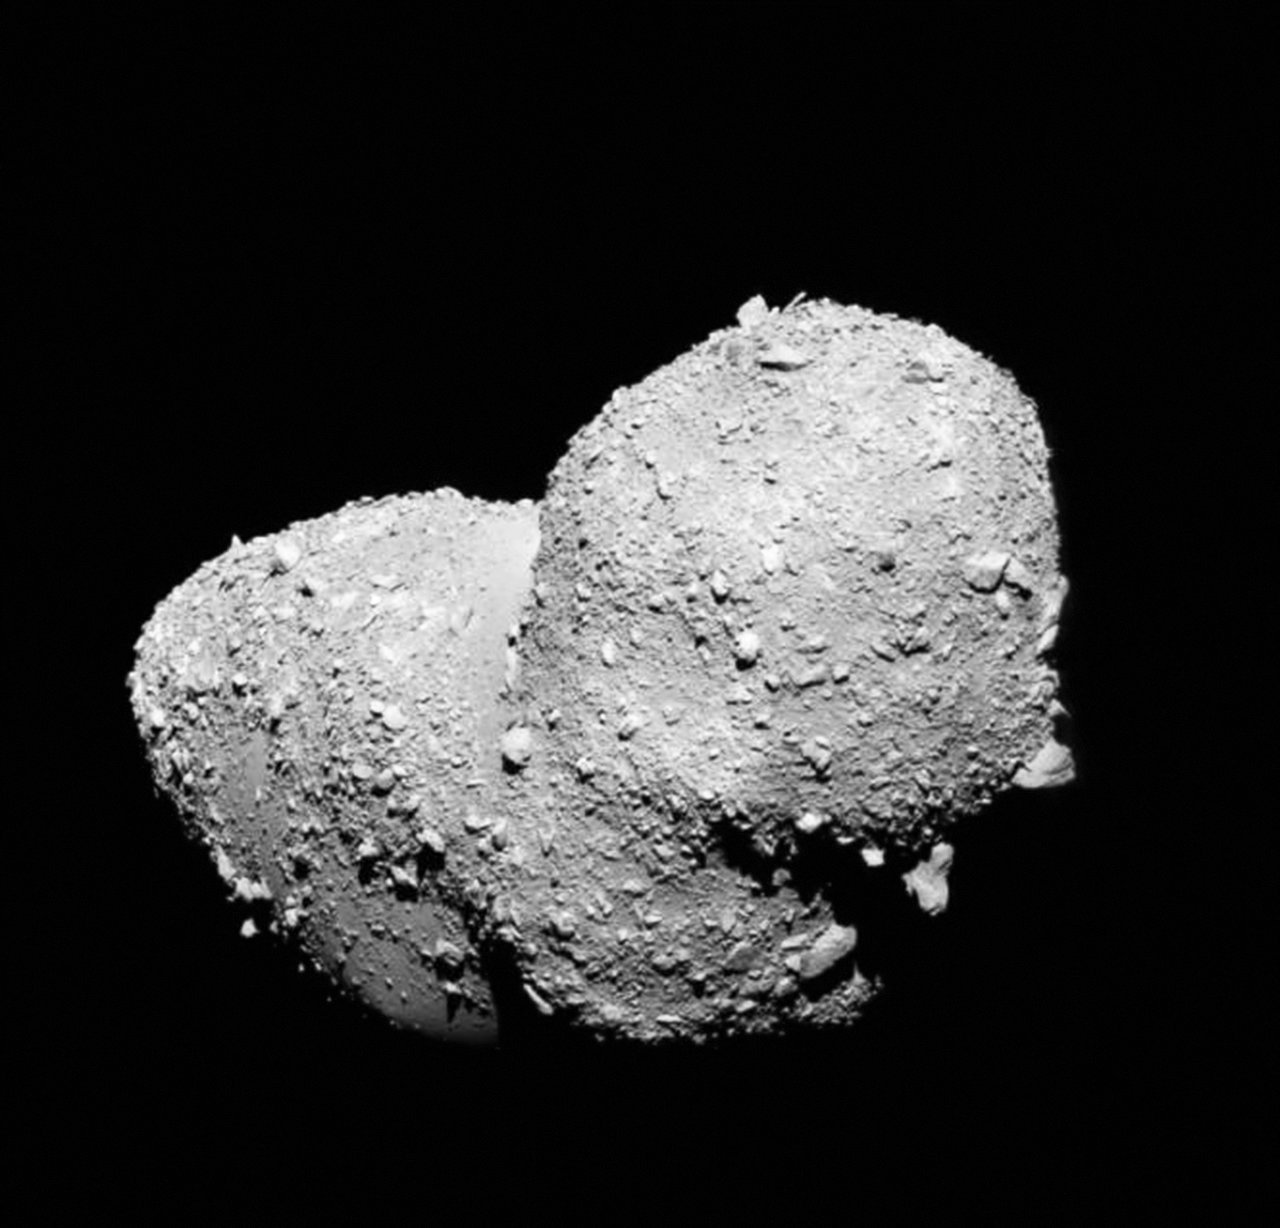
\includegraphics[height=0.3\textheight,width=0.5\textwidth, keepaspectratio]{figures/eso1405b.jpg}}~
    \subcaptionbox{Comet 67/Churyumov-Gerasimenko\label{fig:67p}}{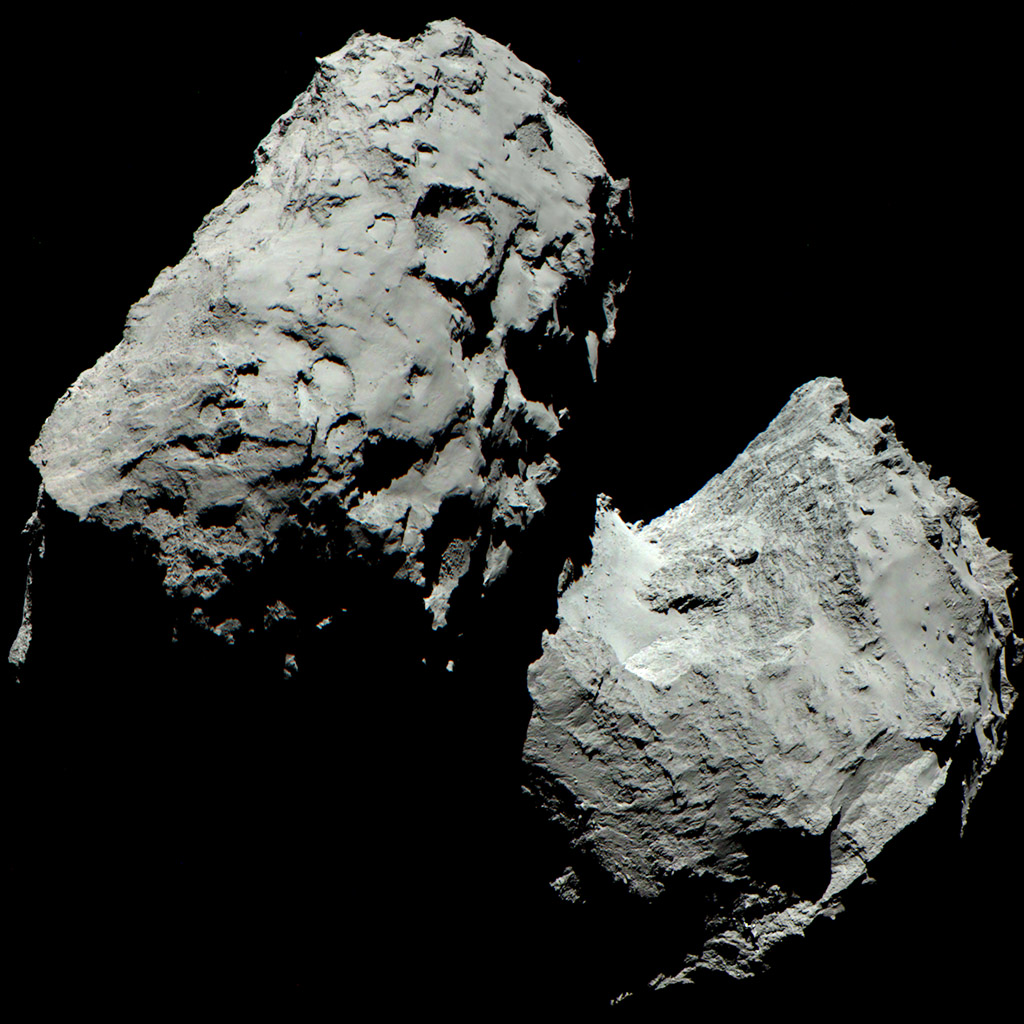
\includegraphics[height=0.3\textheight,width=0.5\textwidth,keepaspectratio]{figures/comet67pcgin.jpg}}
    \caption{Examples of the non-ellipsoidal shapes of small solar system bodies. Both asteroids and comets will tend to have vastly irregular shapes due to their low mass and violent histories of impacts and collisions~\label{fig:irregular_asteroids}}
\end{figure}
The scientific community describes asteroid shape using the facet-vertex model.
This approach is an efficient representation of the more general notion of a polyhedron from geometry.
Here we define the notion of the polyhedron and some specifics of the format used in the astrodynamics community.

A polyhedron is a generalization of a two-dimensional polygon to three-dimensions~\cite{orourke1998}.
It is the region of space with a boundary defined by a surface of a finite number of polygonal faces.
The surface of the polyhedron is composed of three types of primitive objects: zero-dimensional points called vertices, one-dimensional segments called edges, and two-dimensional polygons called faces or facets.
Furthemore, without any loss of generality we assume each face is a convex polygon since any nonconvex face can be divided into smaller convex faces.
A valid polyhedron in the context of asteroid shape models must satisfy several constraints.
These constraints define the relationship between each of the types of primitives which make up the polyhedron surface.
The primitives must intersect ``properly'', the local and global topology must be ``proper''.
For asteroid shape model we further assume that each face is a triangular polygon. 
Again, this does not limit generality as any polygon can be divided into a series of planar triangles.

The intersection of each face must be one of the following:
\begin{itemize}
    \item the faces are disjoint and do not intersect, or
    \item the faces meet at a single vertex, or
    \item the faces share two vertices and a common edge.
\end{itemize}
This constraint automatically ensures that all edgeds and vertices intersect properly.
Improper intersection would penetrating faces and faces that intersect improperly. 
Such as an edge not extending across an entire face.

The second constraint is related to the local topology around each point of the polyhedron.
In order to be locally proper, the neighborhood about any point on the surface of the polyhedron should be homeomorphic to a two-dimensional disk.
A neighborhood about any point on the surface is defined as an arbitrarily small subset or region of the surface which surrounds the point.
Every point on the surface should have a neighborhood which is topologically equivalent to a two dimensional disk.
The notion of equivalency is mathematically captured using the property of homeomorphism.
A homemorphism between two regions is a continous stretching or bending, without tearing or cutting, from one shape to another.
For example, it is possible to turn a circle into a square by a continuous stretching and bending of the shape.
However, it is not possible to transform a sphere into a torus, as this would require a hole to be created in the surface of the sphere.
The neighborhood about any point on the surface of the polyhedron should be equivalent to that of a two-dimensional disk.
A surface where this true for all points is called a \textit{two-manifold}, of a which the surface of a polyhedron is a subset.

The final constraint is related to the global structure of the surface in contrast to the local neighborhood of a point.
The surface must be connected, closed, and bounded.
In this sense, a connected surface is one where it is possible to travel from one point to any other point of the surface without leaving the surface. 
As a result, this will rule out any shapes with non-connected faces, such as a cube with a hollow interior/surface.
For example, on the outer surface of the cube it is not possible to reach a point on the interior surface. 
Combined with an assumption that there are a finite number of faces automatically ensures a closed and bounded surface. 
Note that these conditions do not in general rule out the possibility of holes passing completely through the object.
For example, a torus, or a donute shape, is also considered a polyhedron.
The key difference between a hole and a cavity is that there are no disconnected surfaces and as a result a polyhedron can have any number of such holes. 
In practice, we tend to limit our analysis to polyhedron with no holes, or with a genus of zero.

\subsubsection{Wavefront OBJ files}
The OBJ format is a geometry definition file format used for a variety of computer modeling applications, and is regularly used by the asteroid community~\cite{neese2004}.
The basic format of the file is an ASCII file where the first \( N_v\) lines begin with \texttt{v} and define the three components of a vertex in the body fixed reference frame.
The following \( N_f\) lines begin with \texttt{f} and define the three indices of the vertices that make up the face.
The numbering of the vertices is implicitly defined by the order listed in the file, i.e. the vertices are defined from \( 1 \) to \( N_v\).
There are two main assumptions used by the asteroid community.
First, each face is triangular and second, the vertices are numbered in a counterclockwise fashion about each face.
This allows the outward facing normal to each face to be uniquely defined without any additional data.

\subsection{Shape Reconstruction}

We assume that the spacecraft contains an initial estimate for the shape of the asteroid.
This shape can be a coarse estimate computed from ground measurements or it can be a triaxial ellipsoid based on the semimajor axes of the asteroid, such as that shown in~\cref{fig:start} which represents the maximum axes for asteroid Castalia.
This model is defined as a sequence of vertices, \( \vb{v}_i\), in the asteroid fixed frame and triangular facets, \( f_i = \bracket{\vb{v}_1, \vb{v}_2, \vb{v}_3}\), which are defined by the three vertices making up the facet.
The vertices are assumed to be ordered in a counterclockwise fashion about each facet. 
As a result, the outward facing normal vector to each face is implicitly defined without any additional data.
This shape representation is a widely used format for defining three-dimensional shapes in computer applications and has become the standard method for representing asteroid shapes~\cite{neese2004}.
\begin{figure}
    \centering
    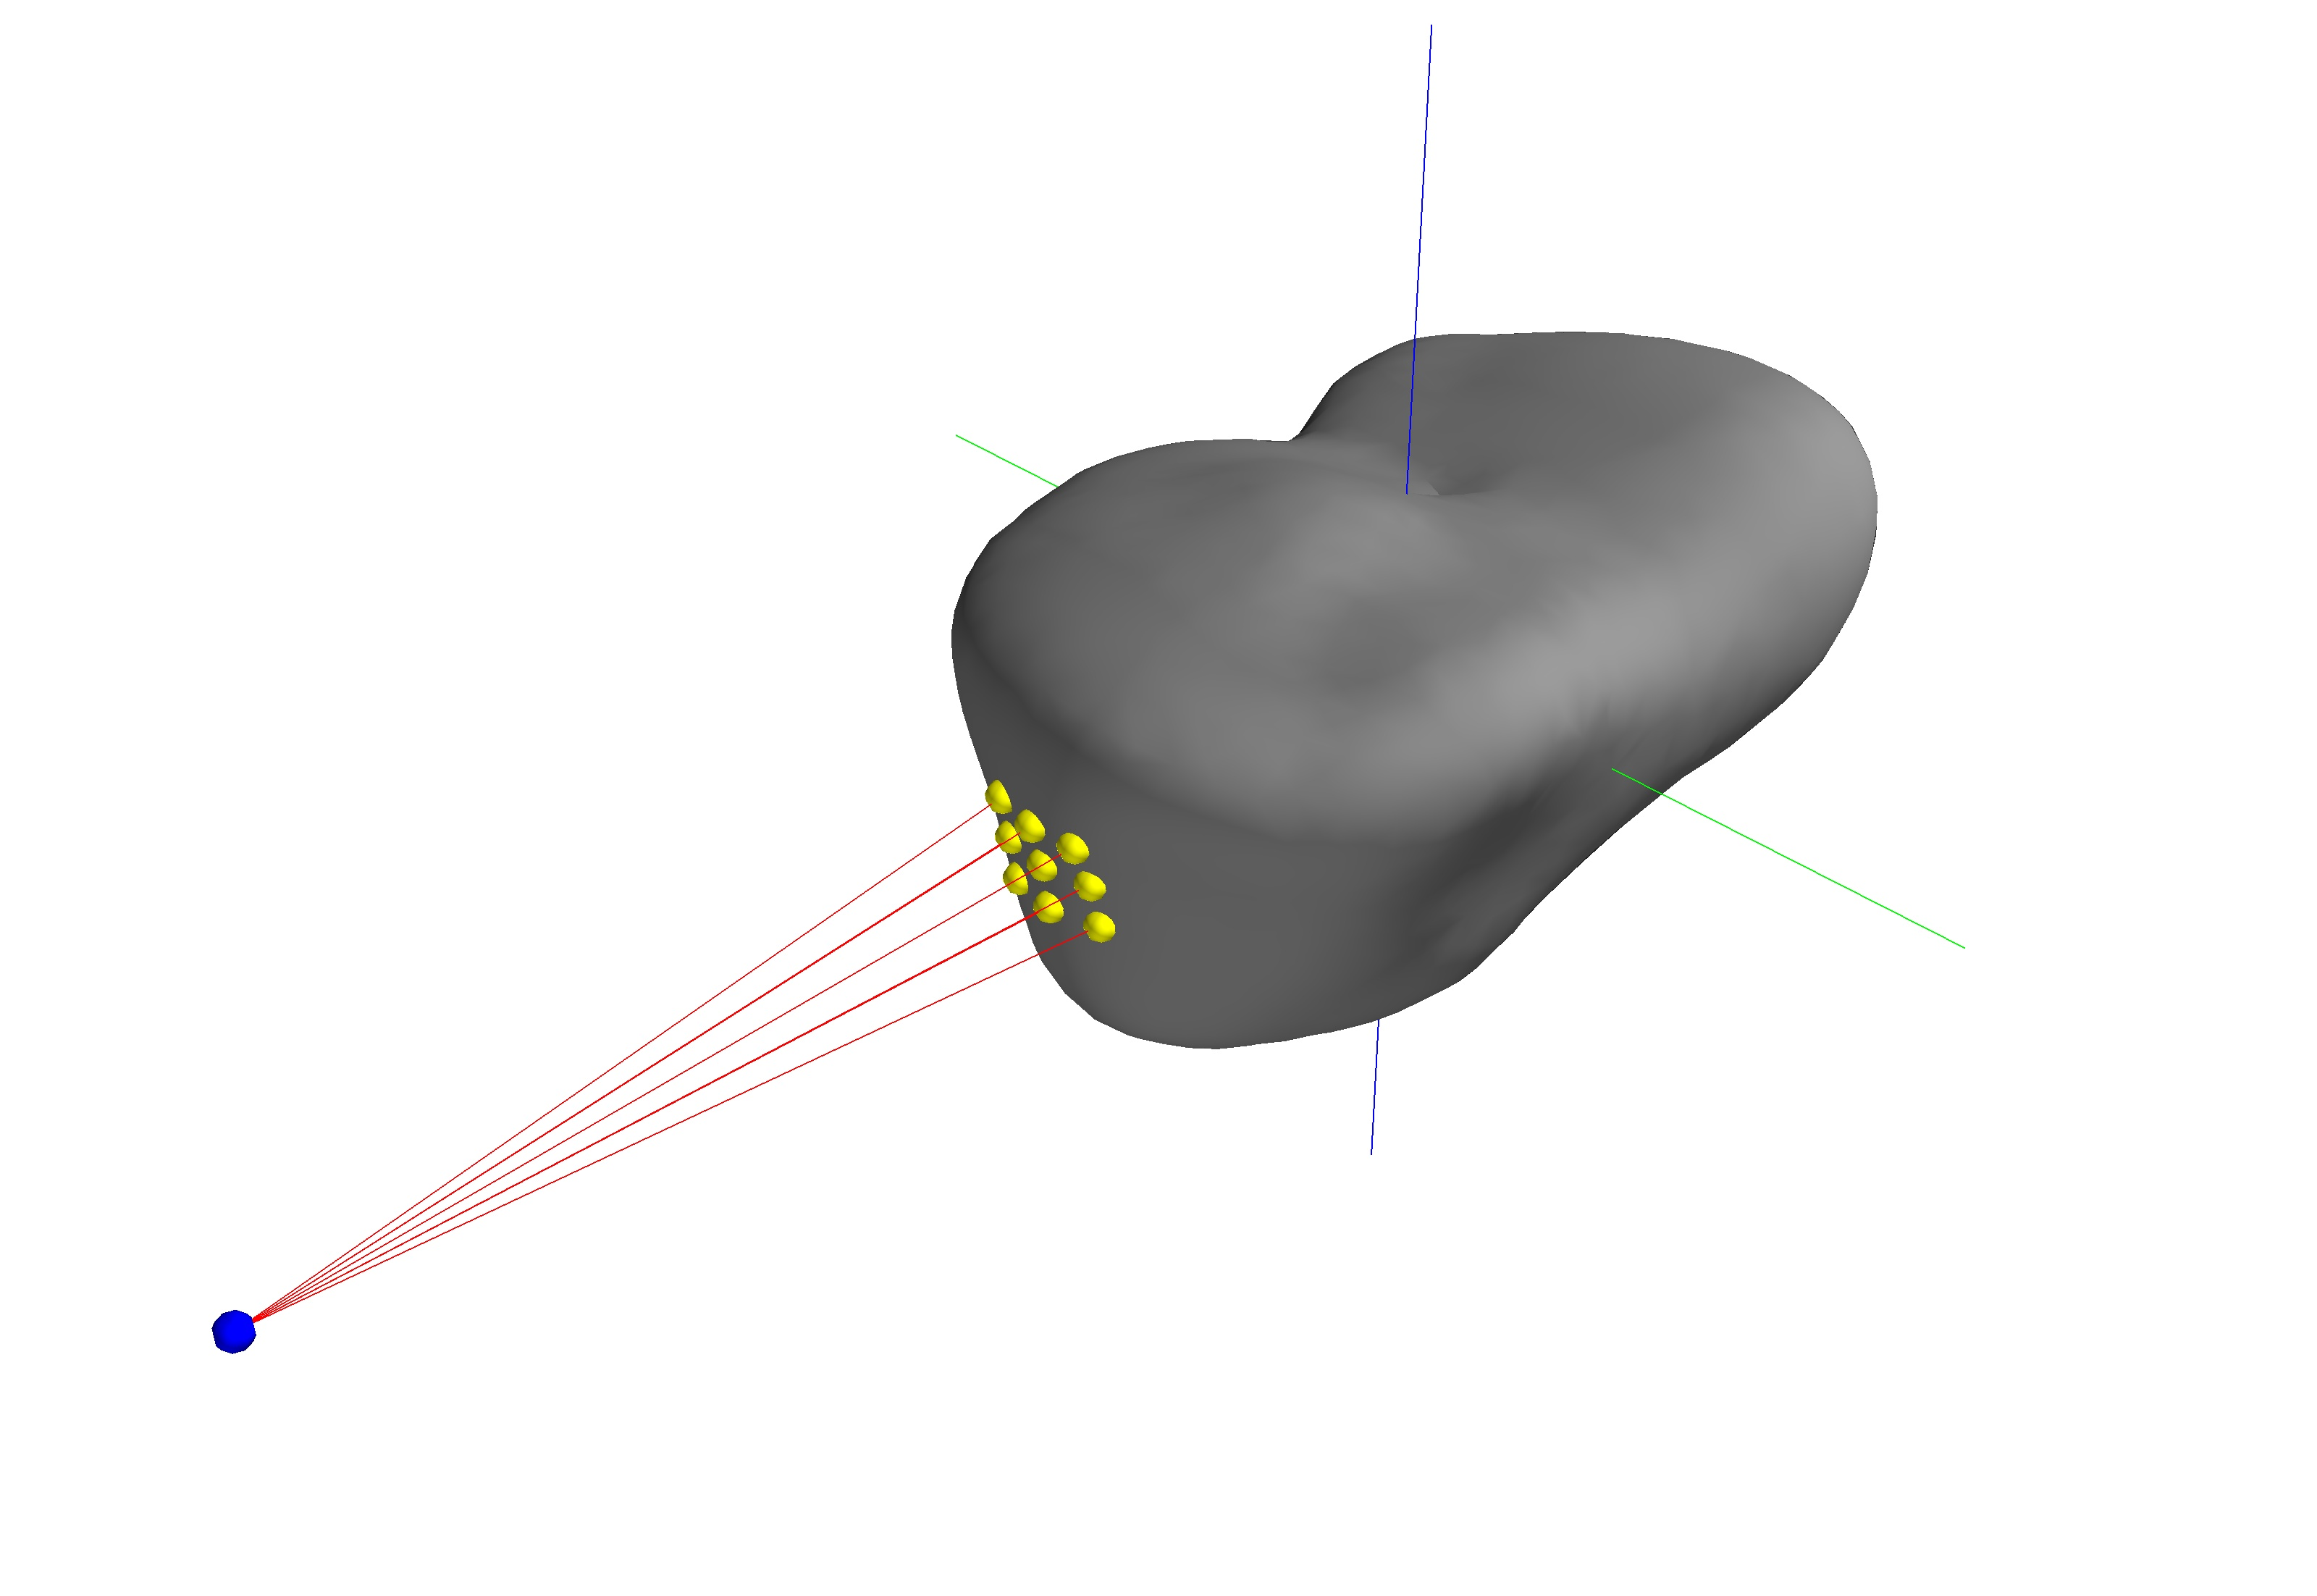
\includegraphics[width=0.75\textwidth]{figures/castalia_raycasting_plot.jpg}
    \caption{Simulated LIDAR measurements of asteroid Castalia~\label{fig:lidar_example}}
\end{figure}

We assume the spacecraft contains a range sensor, such as LIDAR, that allows for the accurate measurement of the relative distance between the spacecraft and asteroid~\cite{zuber1997,zuber2000}.
This type of sensor measures the round-trip time for a pulse of energy to leave the spacecraft, reflect off the surface, and return to a collector on board.
Given the time total time of flight, the distance can be accurately computed using \( d = \frac{\Delta TOF}{2 c} \) where \( c \) is the constant speed of light.
Assuming accurate knowledge of the pointing direction of the spacecraft we can compute a direction from the spacecraft to the measurement location on the surface.
The output of this sensor is a vector, \( \vb{d}_i \), defined in the spacecraft fixed frame which gives the direction to a measurement point on the surface of the asteroid. 
Using the state of the asteroid, we can transform this measurement to the asteroid fixed frame using the simple transformation
\begin{align*}
    \vb{p}_i = R_A^T R \vb{d}_i .
\end{align*}
Given many measurements, \( \vb{p}_i \), of the asteroid surface we can efficiently update our initial shape estimate to that of the true surface.
\Cref{fig:lidar_example} shows asteroid 4769 Castalia and a representation of several LIDAR measurements. 
The spacecraft measures the range between itself and the asteroid surface to several points within the field of view of the sensor. 
These measurements provide a collection of points which lie on the surface of the asteroid, and by combining many points, a so called ``point cloud'', allows us to reconstruct the shape.

Our algorithm applies a Bayesian framework to radially modify each vertex \( \vb{v}_i\) of the shape estimate based on measurement \( \vb{p}_i\). 
This approach alleviates much of complexity of incorporating new vertices or surface triangulation common in surface reconstruction methods~\cite{berg2008}.
This assumption means that the total number of vertices of the shape model is fixed.
However, additional detail, in the form of additional vertices, is possible by using standard mesh subdivision algorithms~\cite{orourke1998}.

The radial distance of each vertex, \( v_i = \norm{\vb{v}_i}\), is assumed to be distributed according to the Gaussian distribution
\begin{align*}
    v_i \sim \mathcal{N}(r_i, w_i^2)
\end{align*}
where \( r_i \) is the initial estimate of the radial distance of vertex \( \vb{v}_i\) and \( w_i \) is the initial variance, or confidence, in the radial distance.
The radial distance of each measurement, \( p_{j,i} = \norm{\vb{p}_j}\), is also assumed to be distributed according to the Gaussian distribution
\begin{align*}
    p_{j,i} \sim \mathcal{N}(r_{j,i}, w_{j,i}^2)
\end{align*}
where \( r_{j,i} = \norm{\vb{p}_{j,i}} \) defines the radial distance of the surface vector measurement and \( w_{j, i}\) defines the variance of the measurement with respect to vertex \( \vb{v}_i\).
Each measurement is defined by the index \( j \) while the associated vertex is defined by \( i \). 
As a result, the measurement \( p_{j, i} \) defines the distribution of measurement \( j \) with respect to vertex \( i \). 
A given measurement may be used to update one or several vertices.

The variance for each measurement vector is assumed to be related to the ``distance'' from the measurement to vertex \( \vb{v}_i \).
Here we use the geodesic distance to parameterize the difference, and hence  uncertainty, of associating the measurement with a given vertex.
From spherical trigonometry the central angle between measurement \( \vb{p}_i \) and vertex \( \vb{v}_i \) of the shape estimate is
\begin{align}
    \Delta \sigma_{j,i} = \arctan \parenth{\frac{\norm{\vb{p}_j \times \vb{v}_i}}{\vb{p}_j \cdot \vb{v}_i }}.
\end{align}
The variance of measurement \( \vb{p}_i \) with respect to vertex \( \vb{v}_i \) is then defined as the arc length as
\begin{align}
    w_{j, i} = \norm{\vb{p}_j} \Delta \sigma_{j,i} .
\end{align}
This approach relates the uncertainty of the measurement, \( \vb{p}_j \) with the geodesic distance to a given vertex, \( \vb{v}_i \).
As a result, measurements which are far from a vertex, where \( \Delta \sigma \) is large, will tend to have a larger variance and hence uncertainty. 
From Bayes' theorem, the posterior probability is
\begin{align}
    p(v_i | p_{j, i}) = \frac{p(p_{j, i} | v_i) p(v_i)}{p( p_{j, i})} \propto p(p_{j,i} | v_i) p(v_i).
\end{align}
From the properties of a Gaussian, the posterior probability given a measurement is also distributed according to a Gaussian distribution~\cite{bishop2006} and given by
\begin{align}\label{eq:posterior_probability}
    \mathcal{N} \parenth{\frac{w_{j, i}^2 r_i + w_i^2 r_{j, i}}{w_i^2 + w_{j, i}^2} , \frac{w_i^2  w_{j, i}^2}{w_i^2 +  w_{j, i}^2}} .
\end{align}
From~\cref{eq:posterior_probability}, the posterior probability conditioned on the measurement is the weighted average of the prior knowledge and the measurement. 
Measurements that are far from the vertex will have a high uncertainty or variance and will have a reduced impact on the radial position of the vertex.
Additional measurements are incorporated using a weighted average of prior belief and the measurement uncertainty.

In order to improve the computational efficiency measurement updates are assumed to be local in nature.
Instead of applying a measurement to all vertices of the mesh, the measurement is only applied to the vertices which are within a specified region of the measurement. 
We define a region of interest, \( \Delta S \), about each measurement which defines the surface area over which the measurement will affect the mesh estimate.
We relate \( \Delta S \) to an equivalent angular constraint using
\begin{align}
    \Delta \sigma_{max} = \sqrt \frac{\Delta S}{r_b^2}
\end{align}
where \( r_b \) defines the Brillouin  sphere radius, or the radius of the circumscribing sphere of the asteroid.
Only vertices which satisfy \( \Delta \sigma_i \leq \Delta \sigma_{max} \) are considered in the Bayesian update shown in~\cref{eq:posterior_probability}.

\section{Preliminary Results}
\begin{figure}[h]
    \centering
    \subcaptionbox{Initial mesh estimate\label{fig:start}}{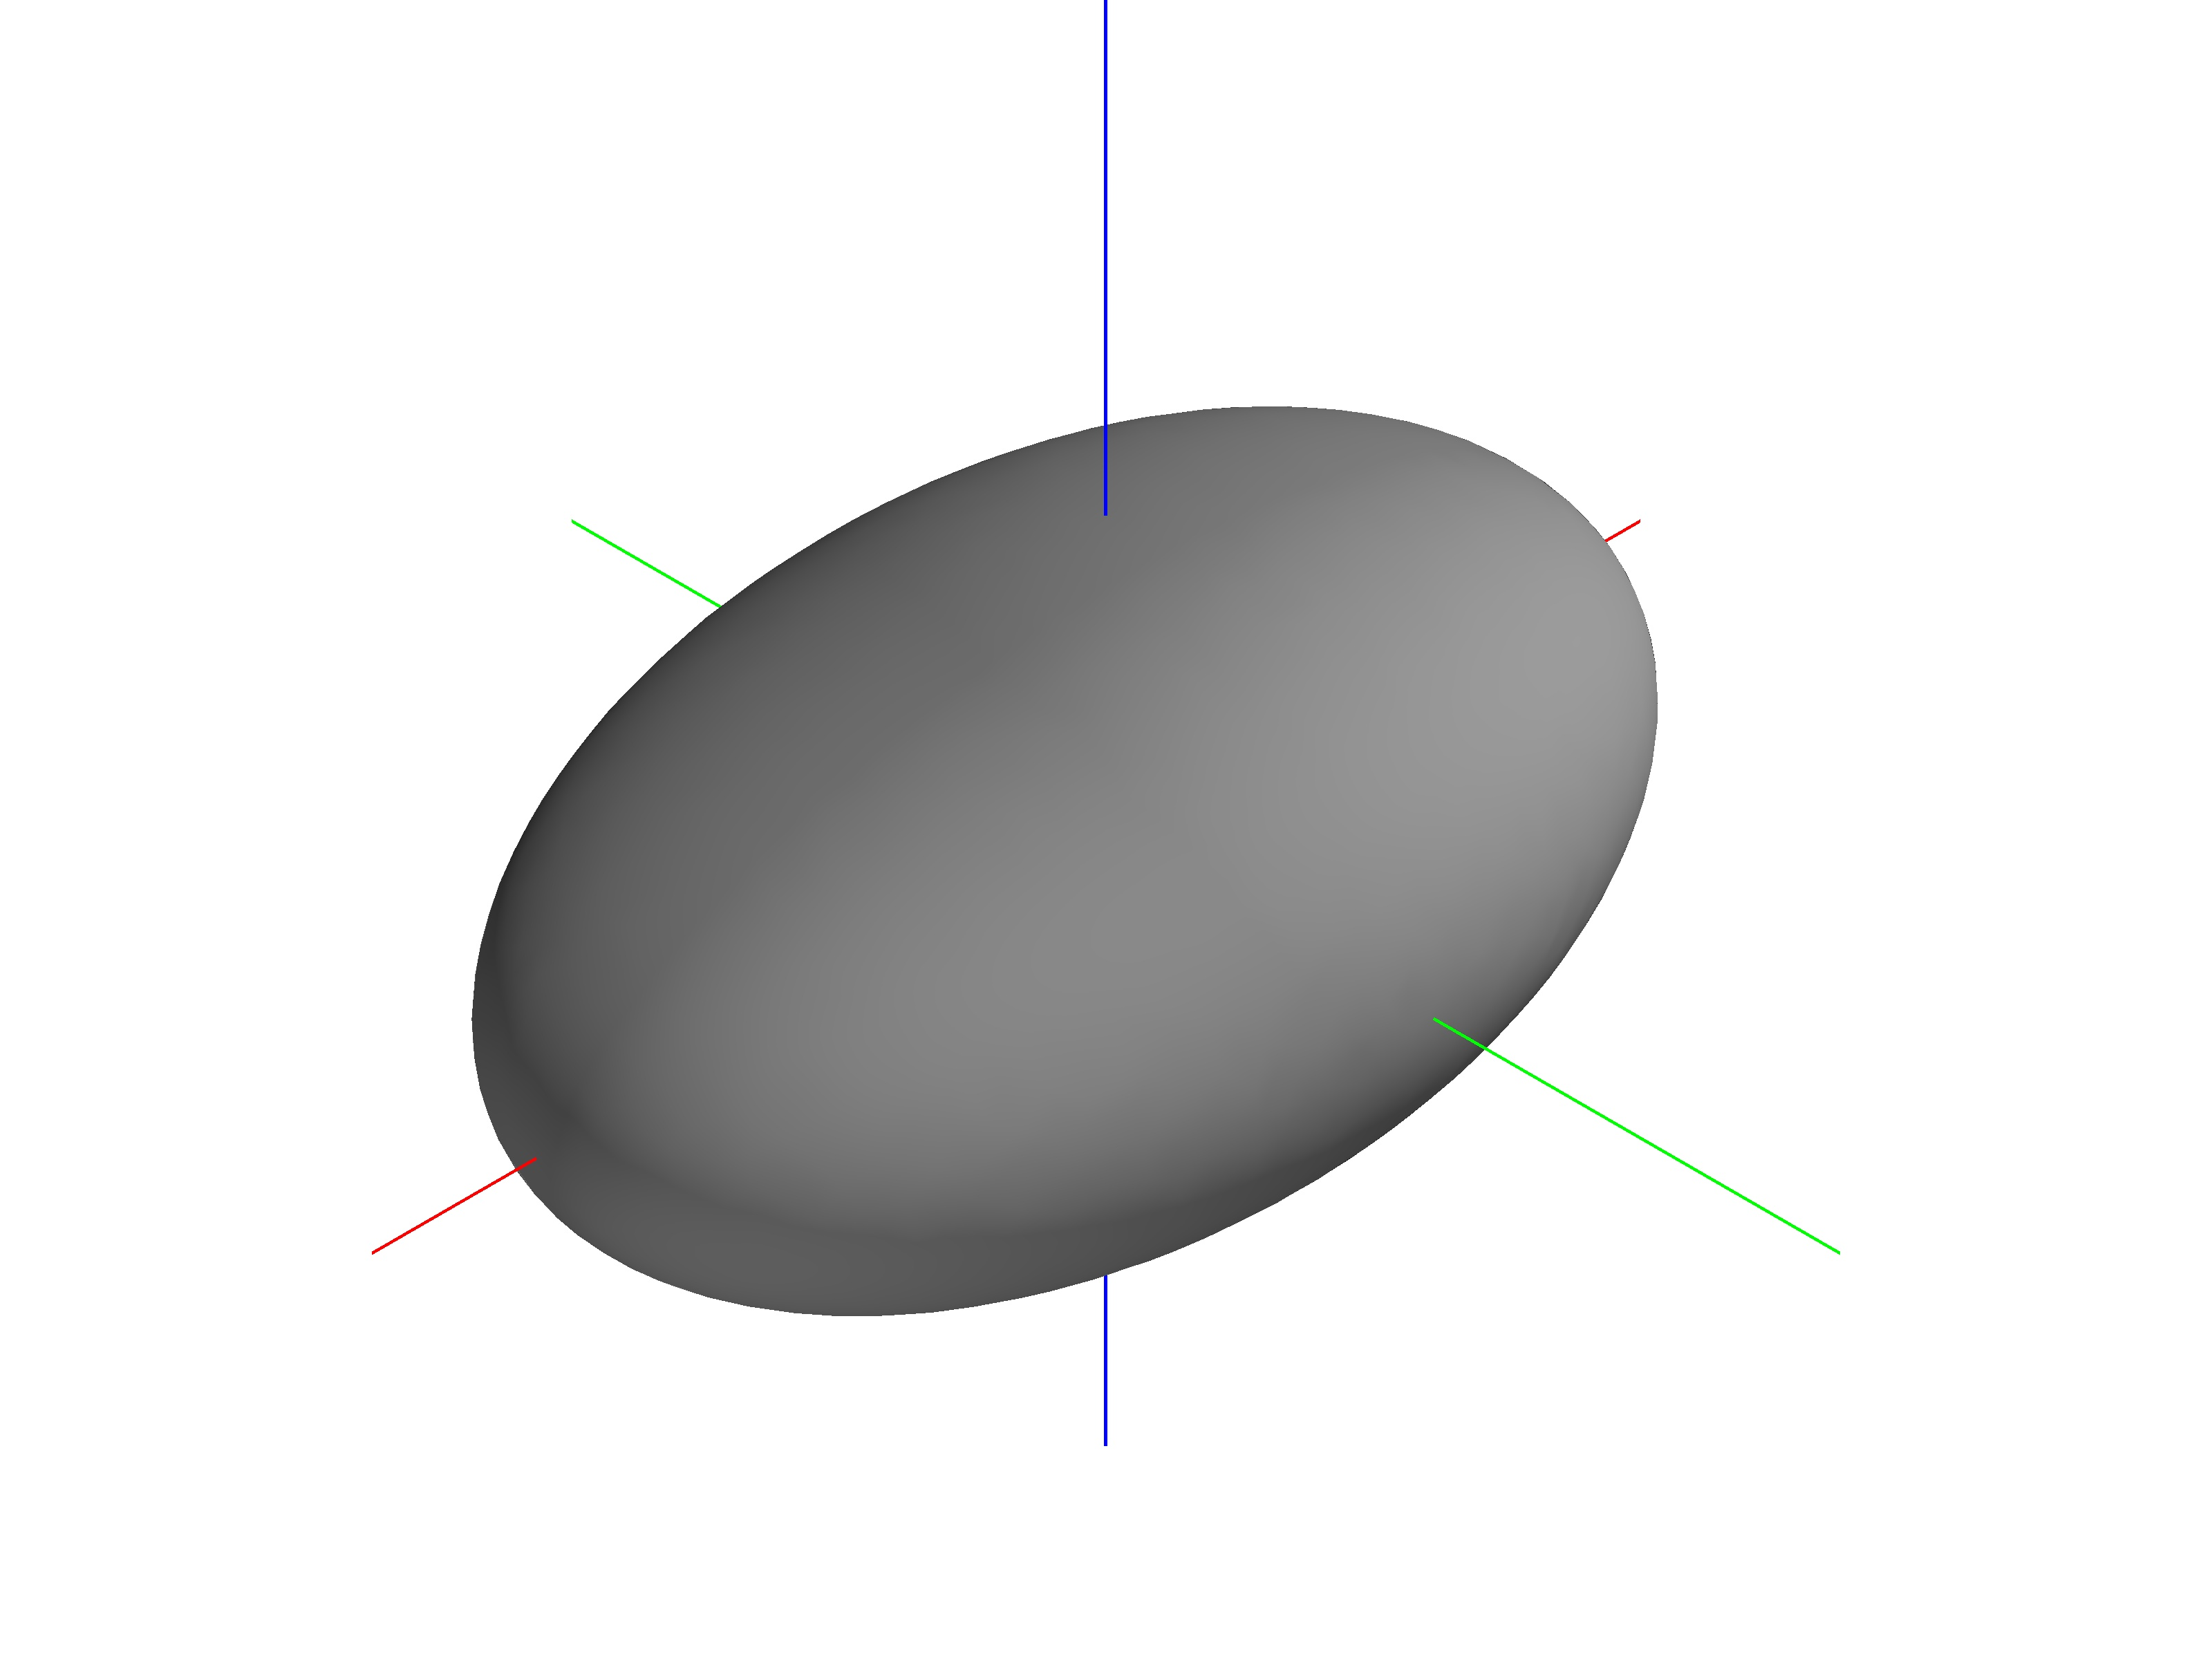
\includegraphics[height=0.5\textheight,width=0.5\textwidth,keepaspectratio]{figures/partial_initial.jpg}}~
    \subcaptionbox{First measurement added\label{fig:first}}{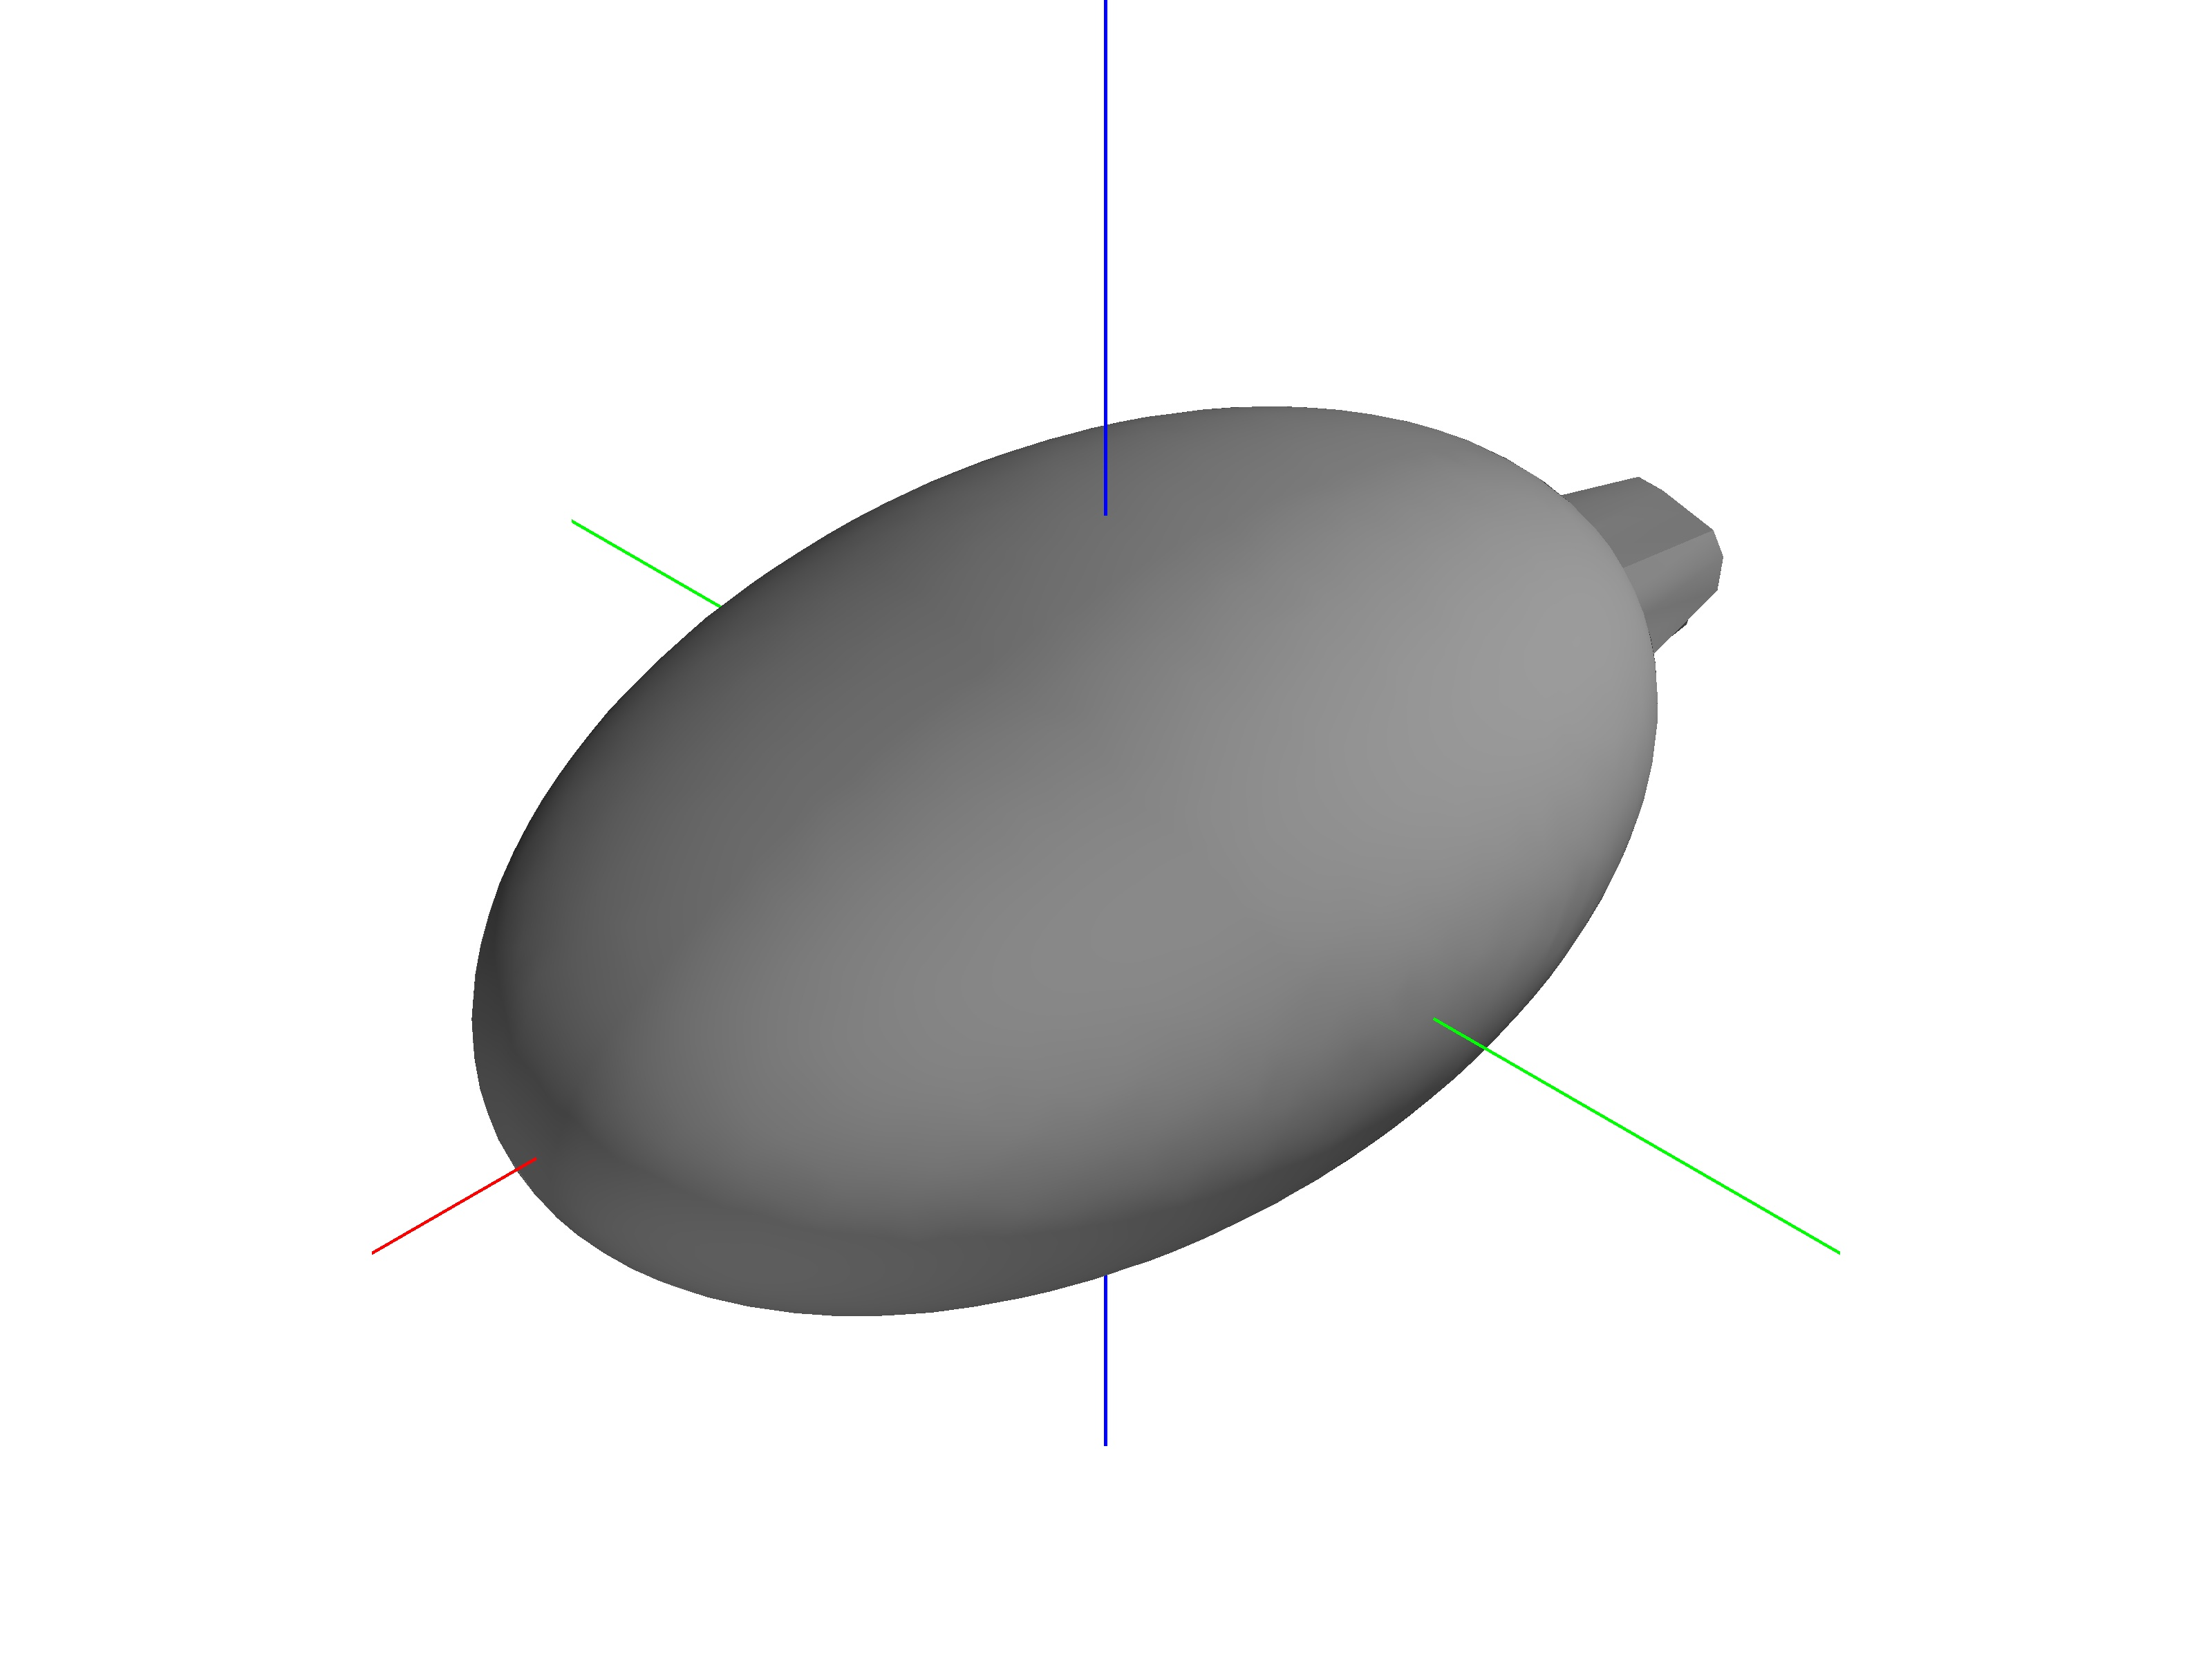
\includegraphics[width=0.5\textwidth]{figures/partial_0.jpg}}

    \subcaptionbox{\SI{25}{\percent} of measurments added\label{fig:quarter}}{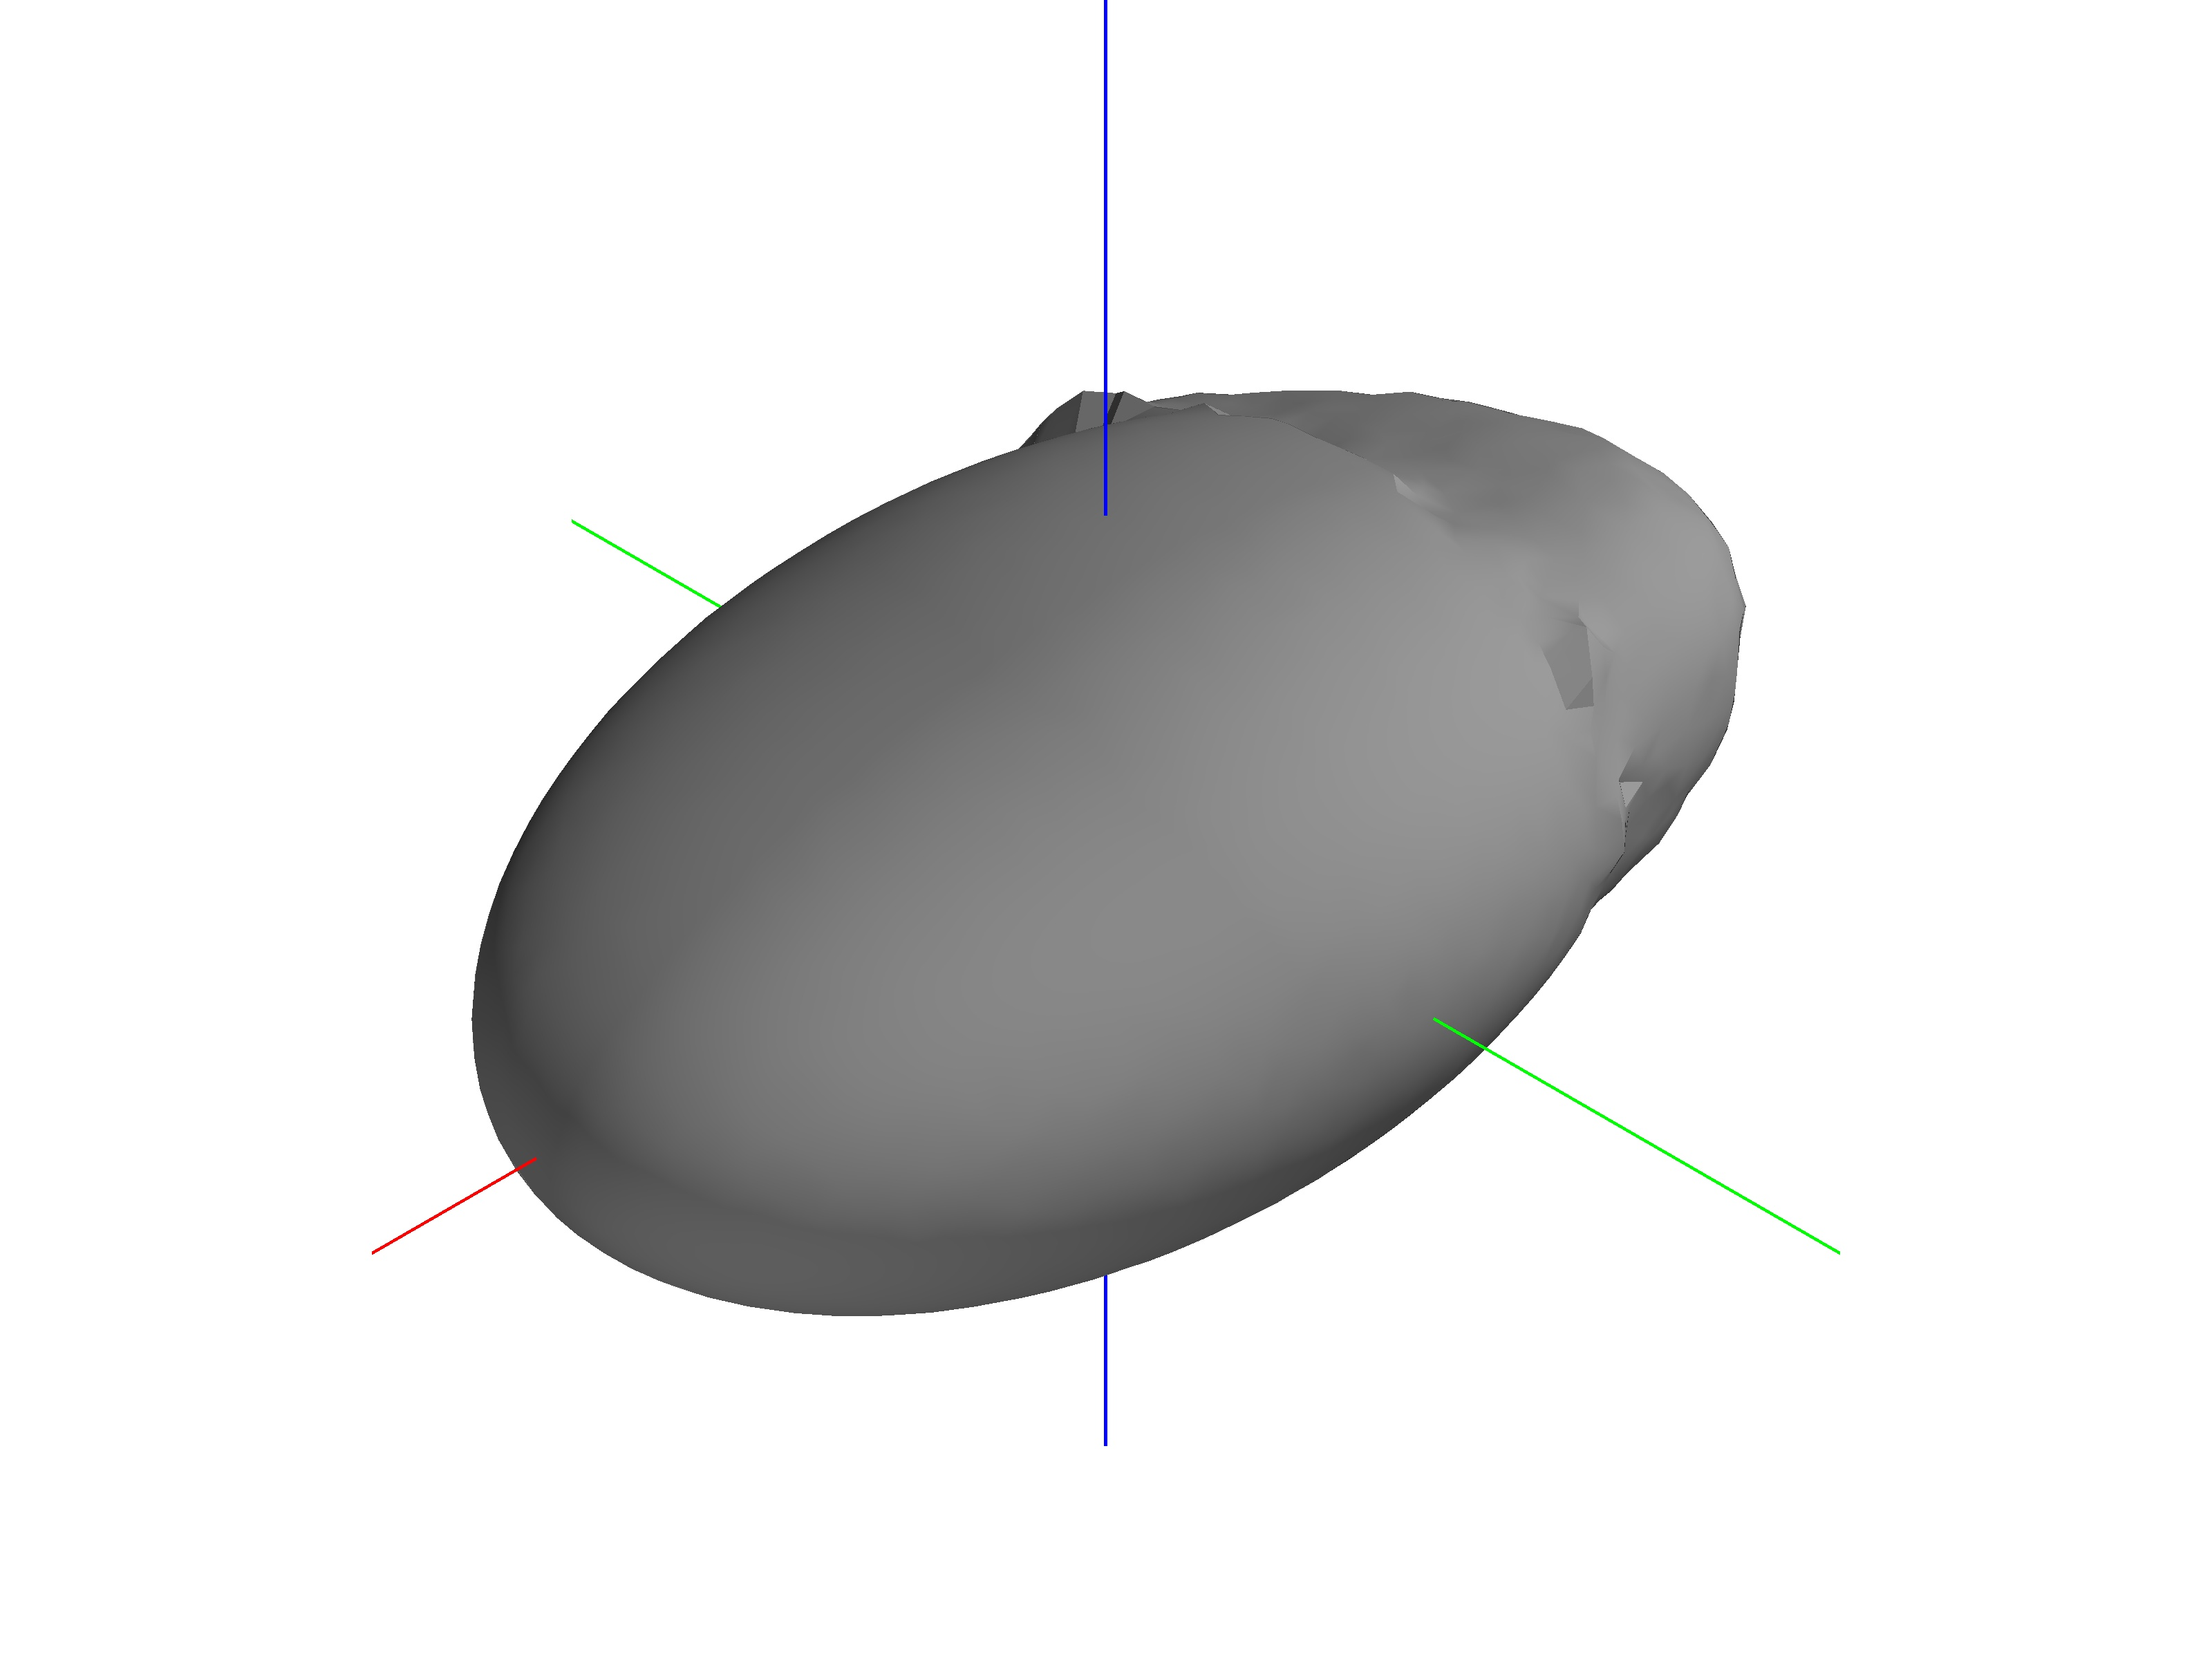
\includegraphics[width=0.5\textwidth]{figures/partial_512.jpg}}~
    \subcaptionbox{\SI{50}{\percent} of measurements added\label{fig:half}}{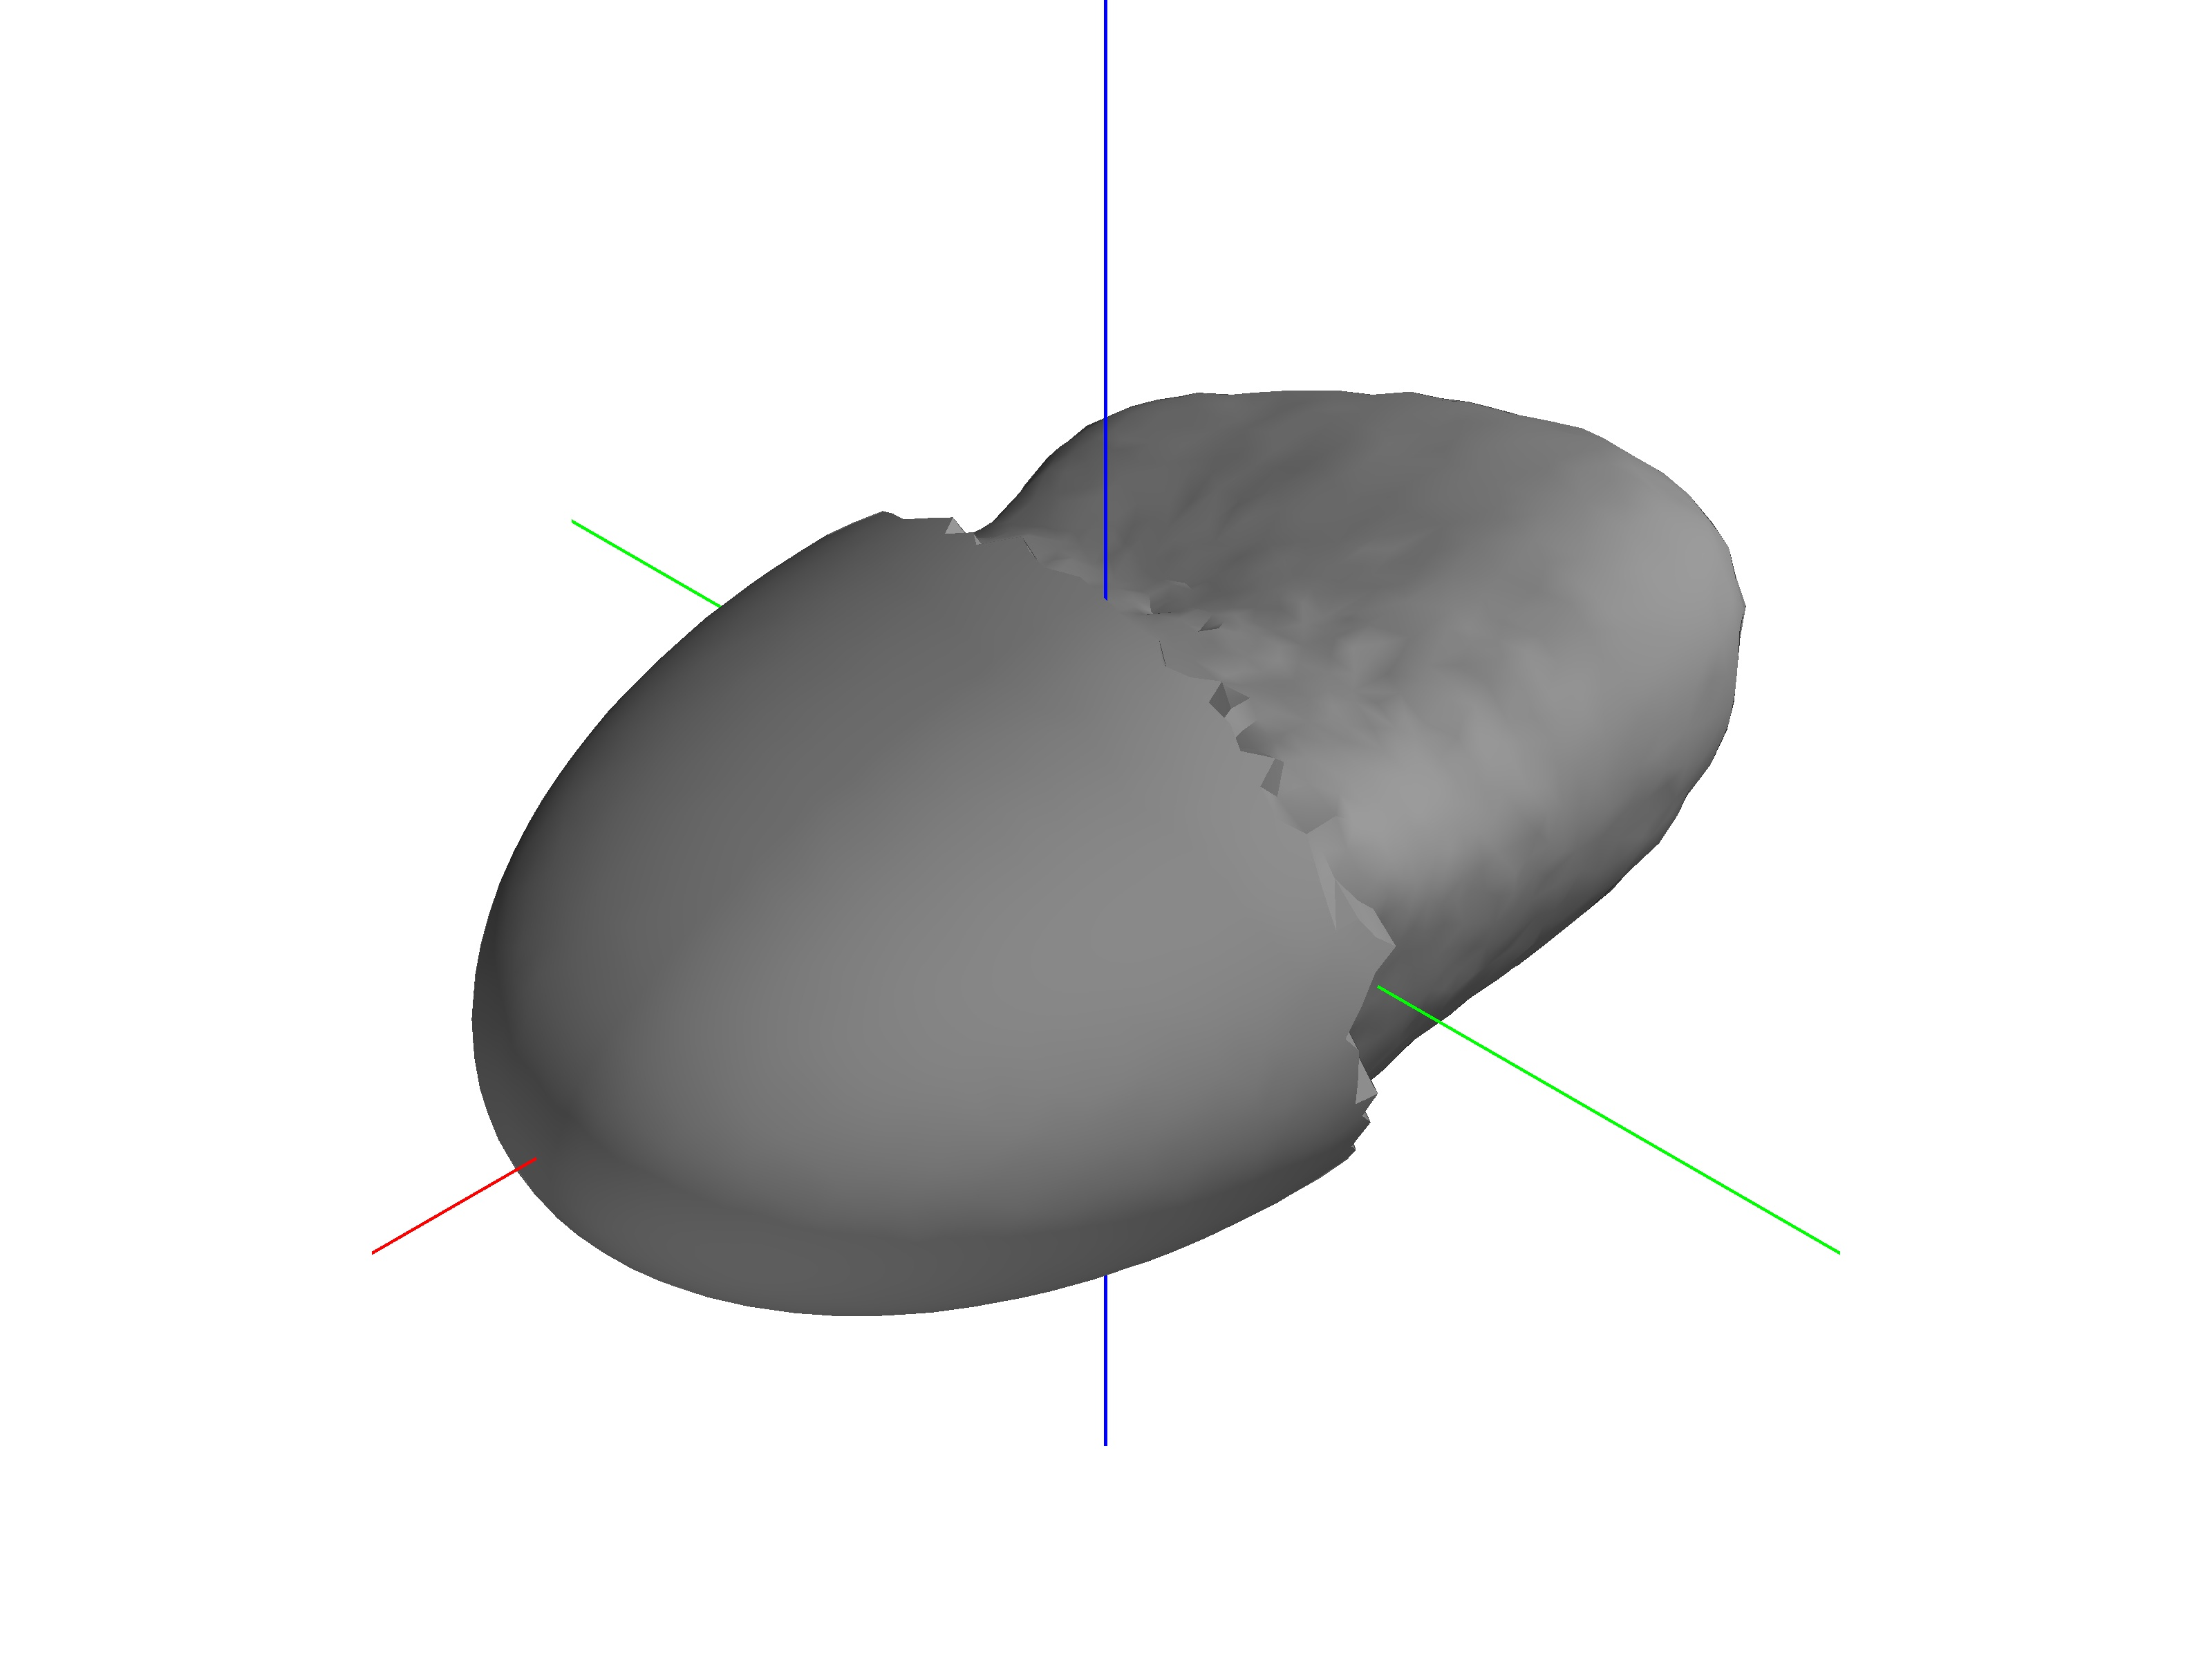
\includegraphics[width=0.5\textwidth]{figures/partial_1024.jpg}}

    \subcaptionbox{\SI{75}{\percent} of measurements added\label{fig:threequarter}}{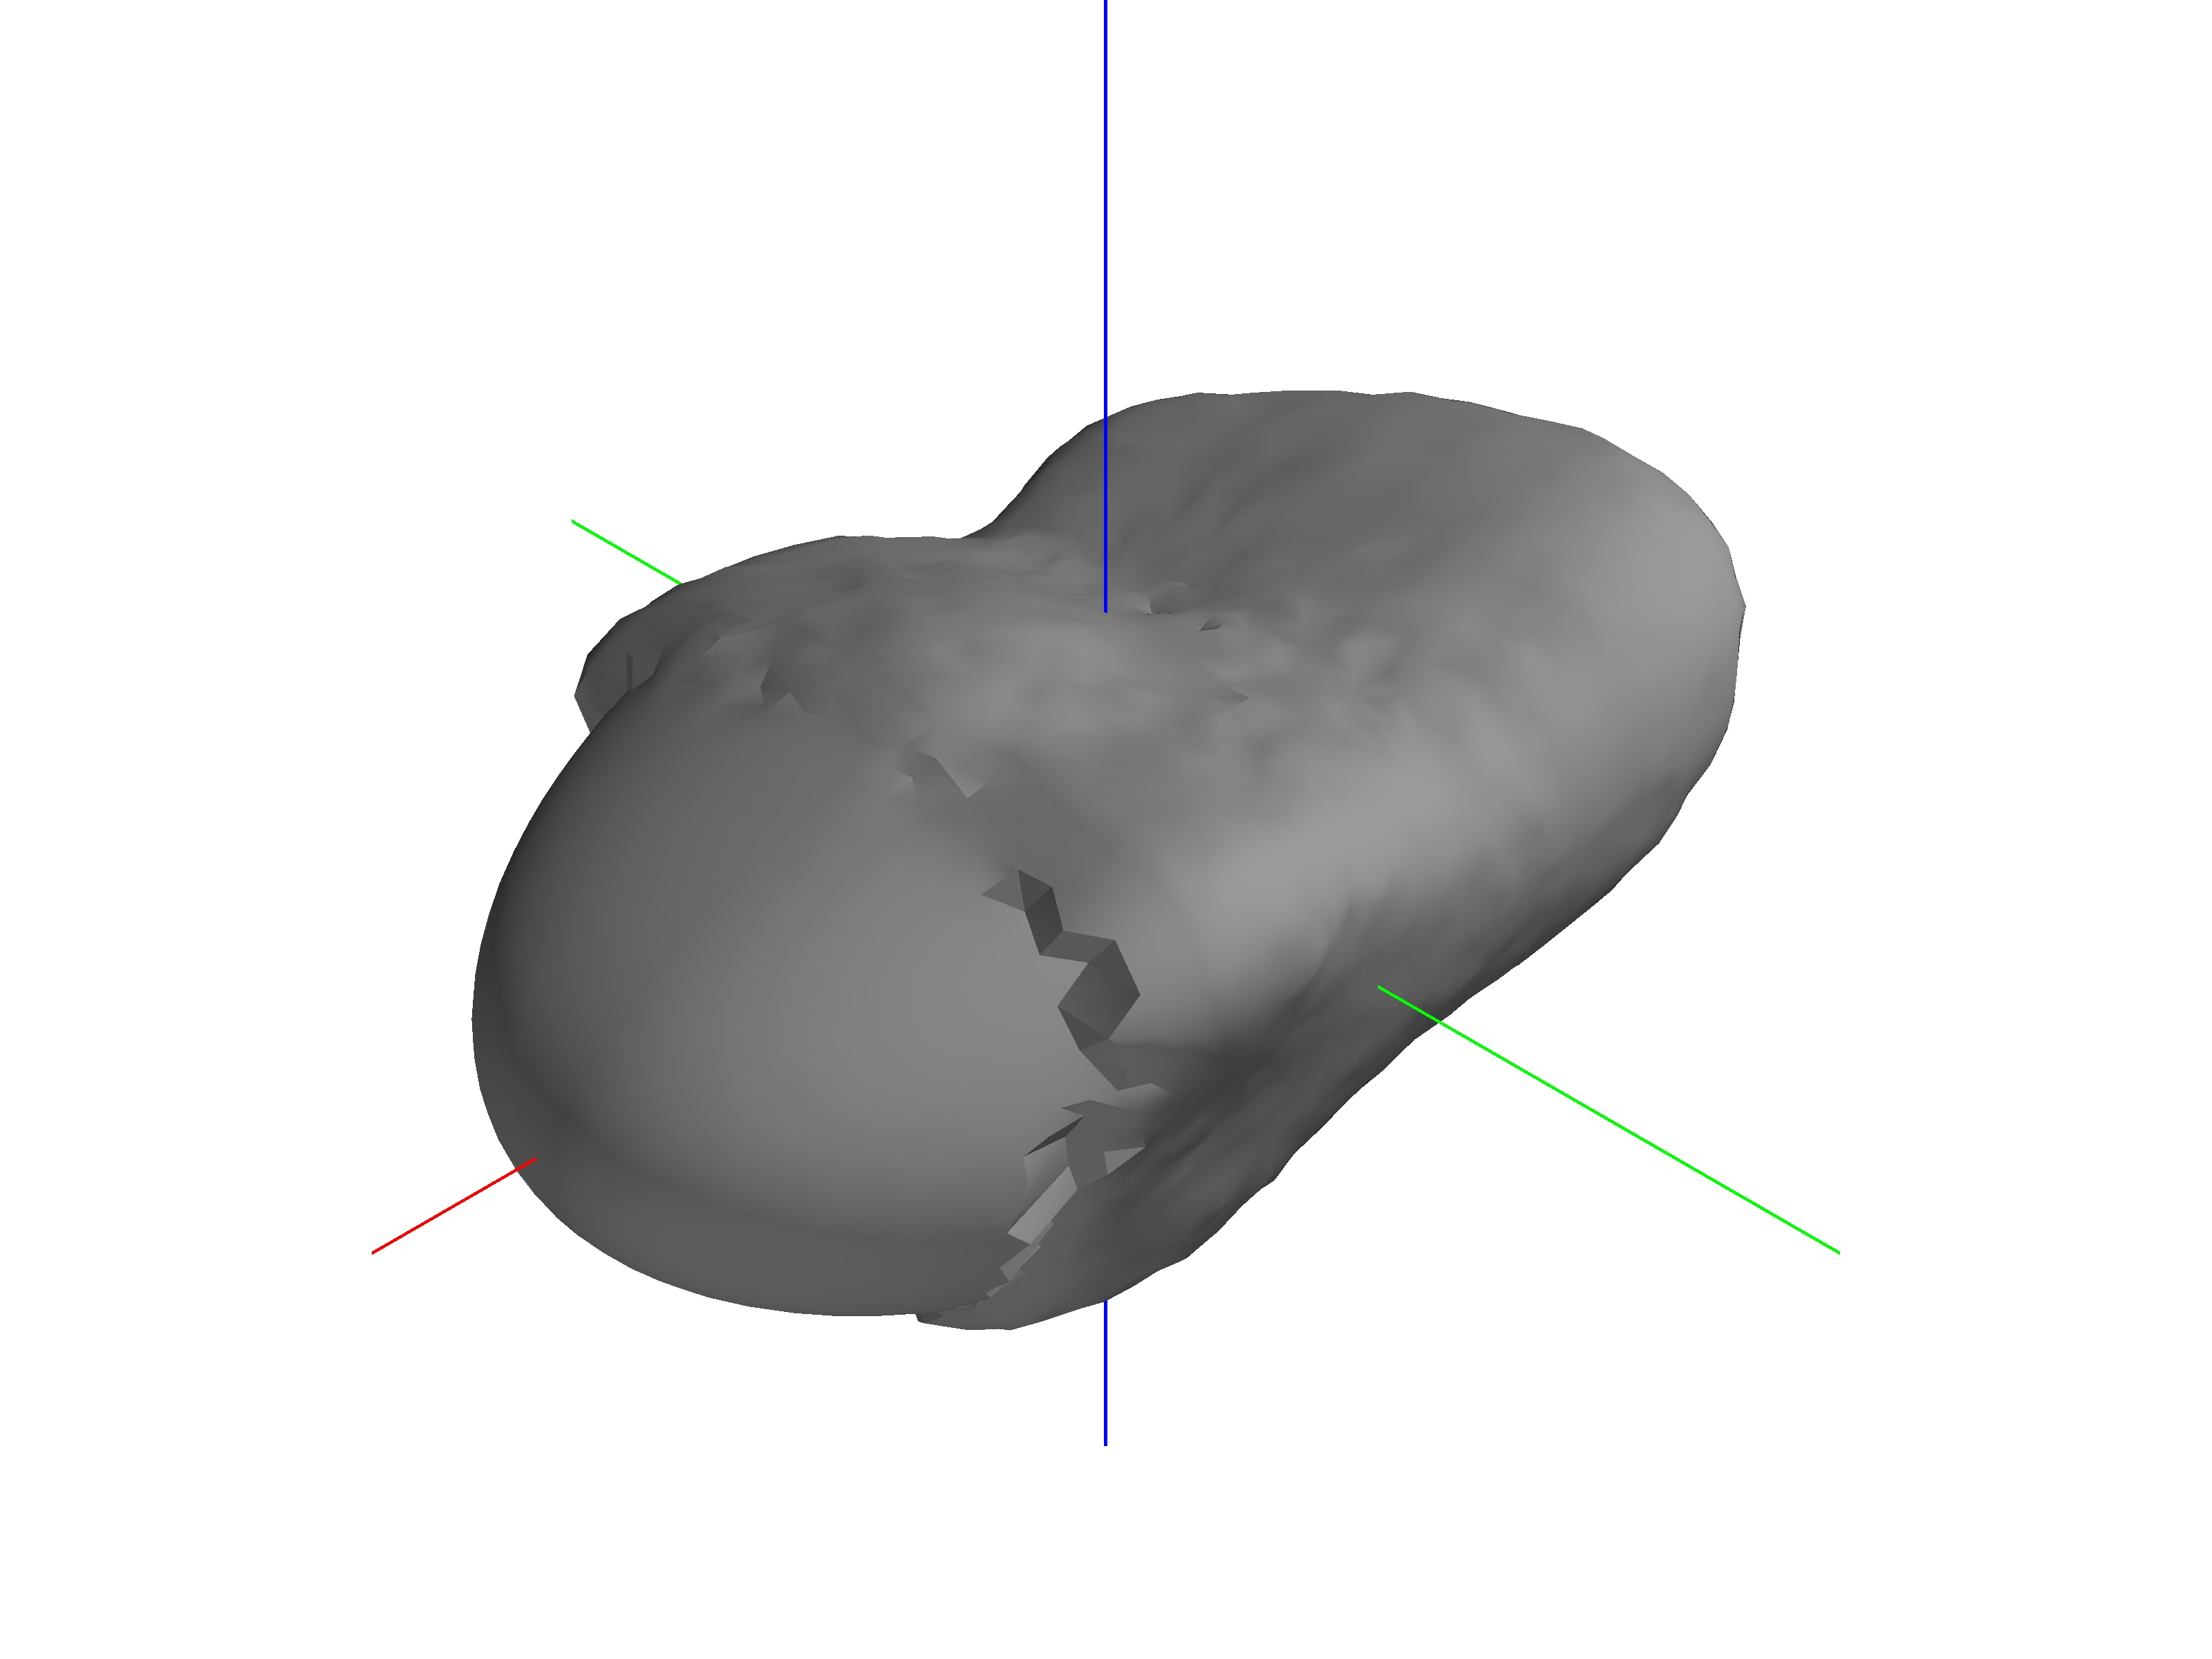
\includegraphics[width=0.5\textwidth]{figures/partial_1536.jpg}}~
    \subcaptionbox{Final reconstruction\label{fig:final}}{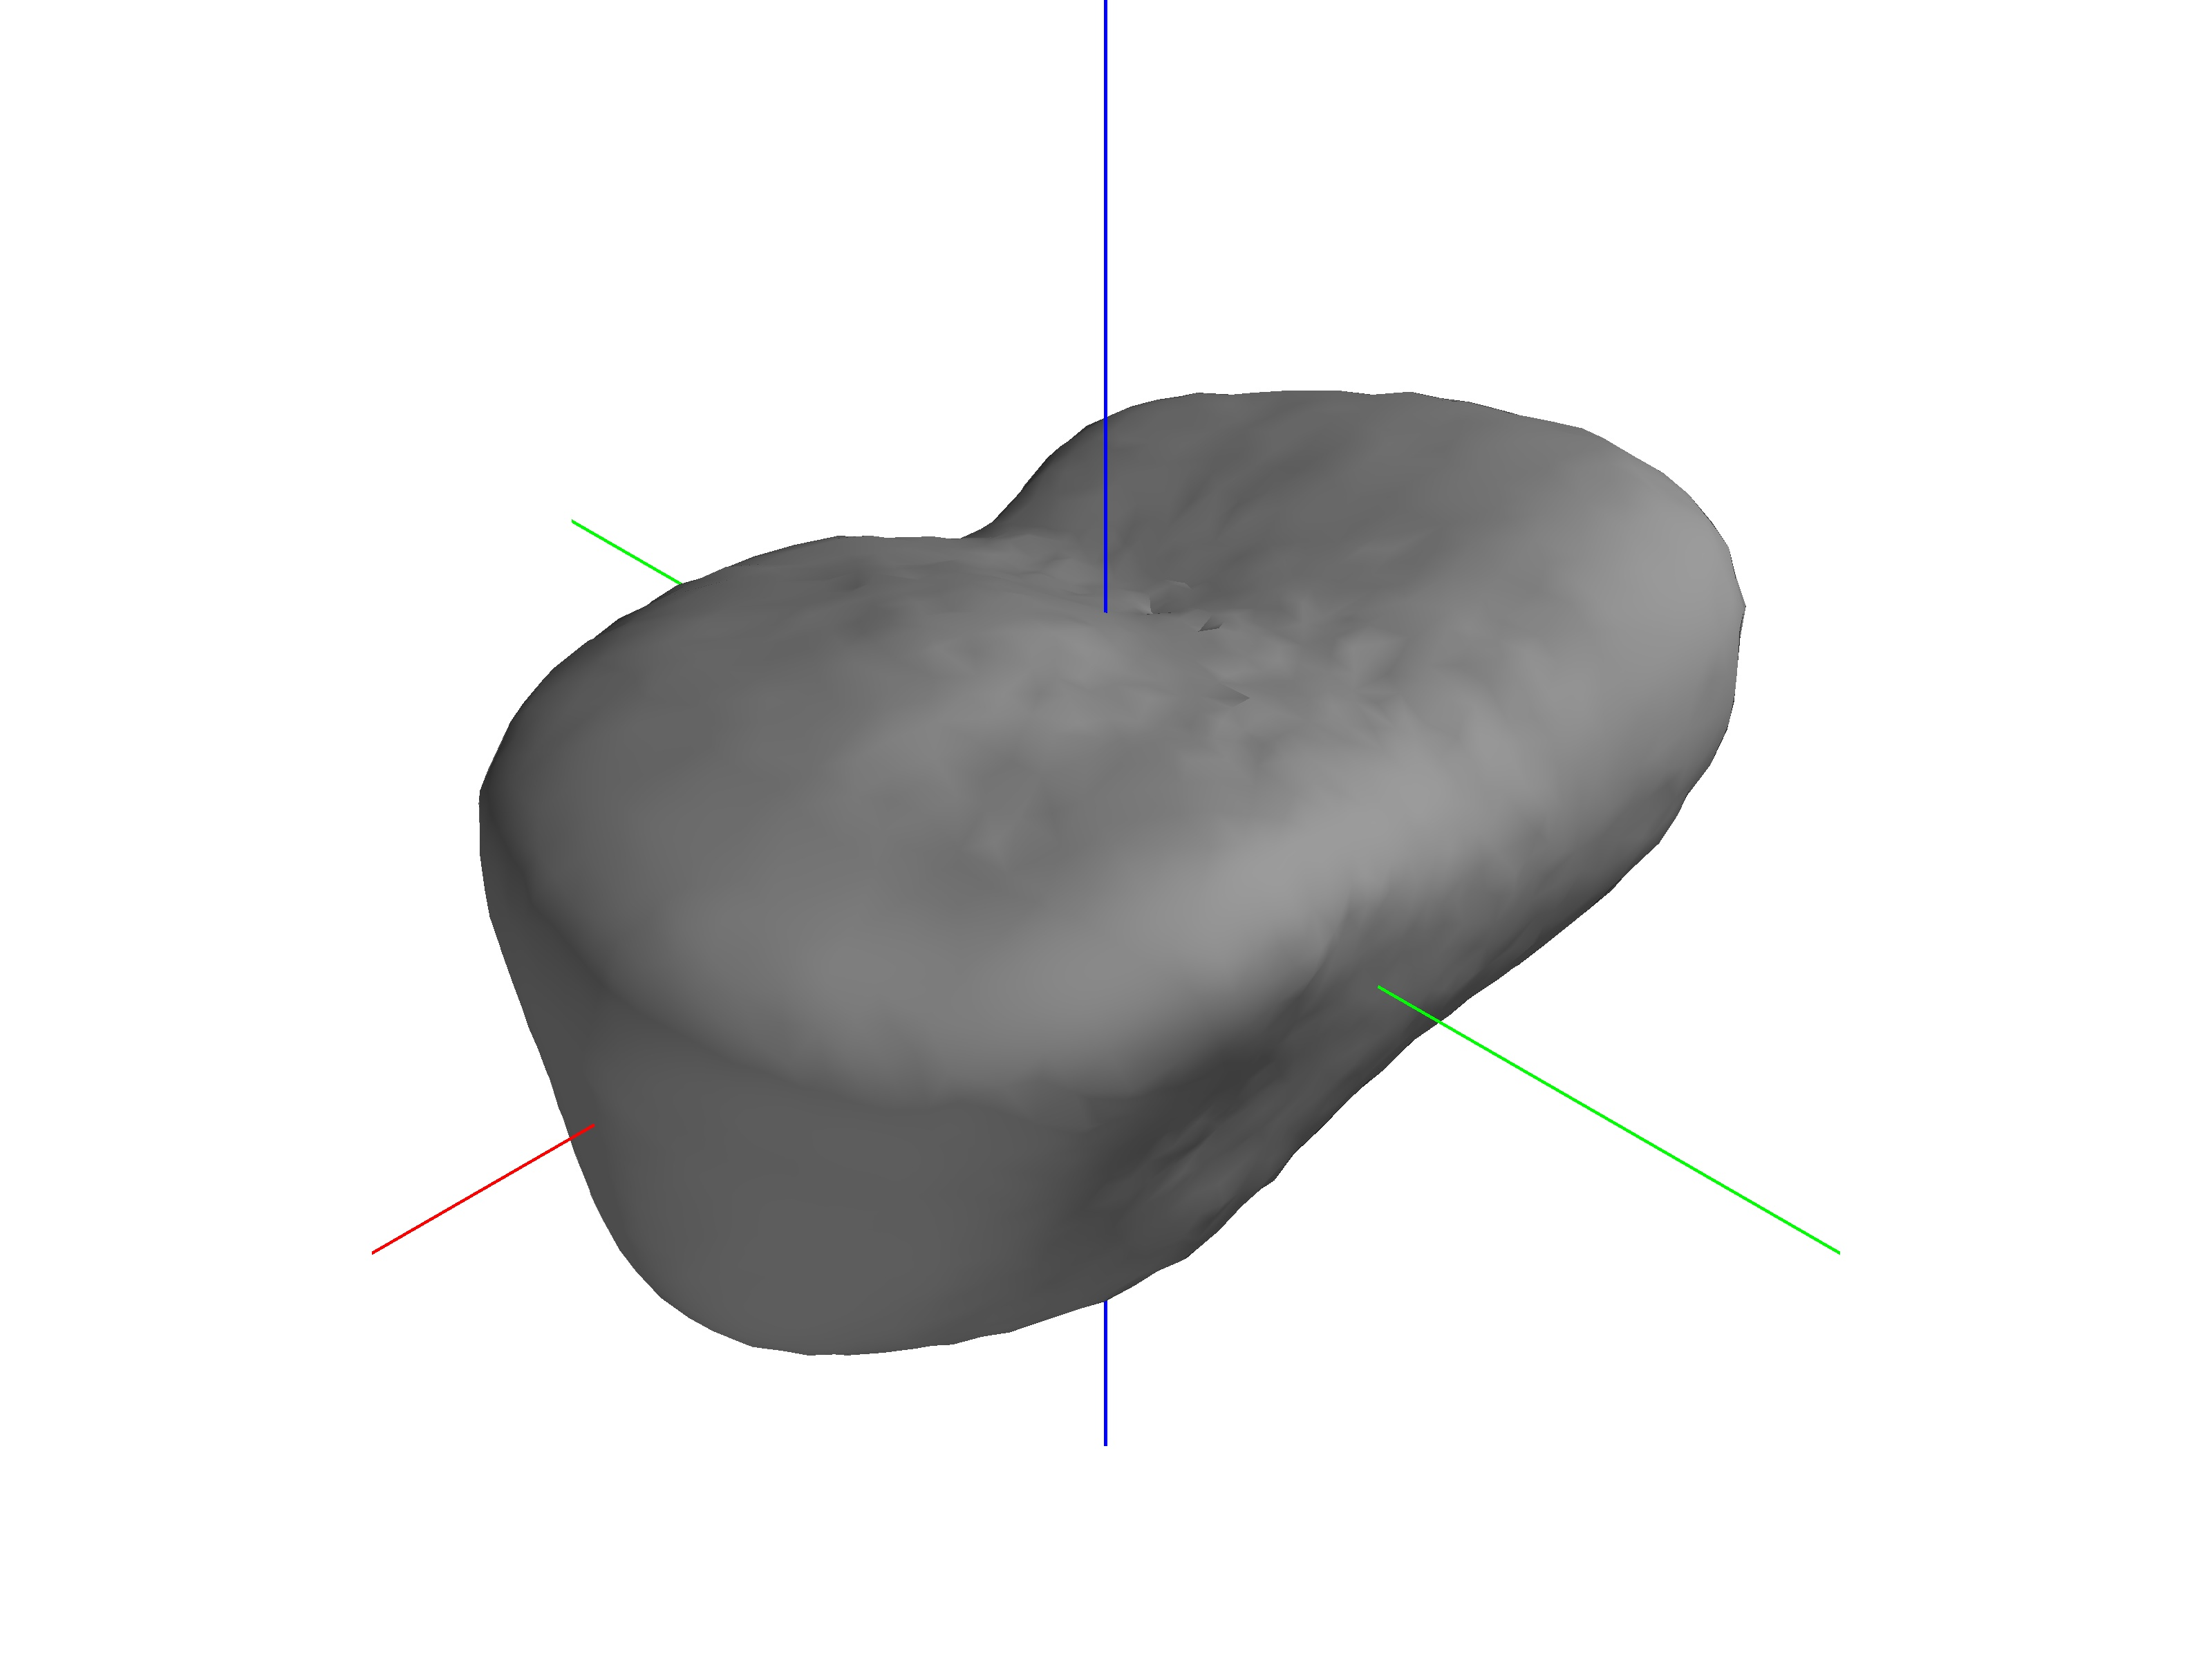
\includegraphics[width=0.5\textwidth]{figures/partial_2047.jpg}}
    \caption{4769 Castalia incremental reconstruction. The initial ellipsoid is incrementally modified by radially moving each vertex to best match the measurements.~\label{fig:reconstruction}}
\end{figure}
Here we present initial results of reconstructing the shape of asteroid 4769 Castalia.
Castalia is a potentially  hazardous asteroid and the first asteroid which used radar imaging to generate a 3D surface shape~\cite{hudson1994}.
In this example, we seek to incrementally build an accurate shape of Castalia from an initial triaxial ellipsoid model.
Our initial shape for Castalia is a triaxial ellipsoid with semi-axes equal to \( \SI{1.8}{\kilo\meter} \times \SI{0.8}{\kilo\meter} \times \SI{0.8}{\kilo\meter}\) and shown in~\cref{fig:start}.
We use this choice of initial estimate since the semi-major axes of an asteroid are able to be computed based on Earth-measurements~\cite{busch2011}.
Furthermore, this type of model also allows for the use of analytical gravitational models for use in preliminary analysis or in the absence of higher fidelity shape information~\cite{scheeres1994}.

Simulated measurements of the surface of 4769 Castalia are used to update the initial mesh estimate.
The truth shape model, and the associated vertices, are used as simulated measurements of the shape of Castalia~\cite{neese2004}.
The true shape model of 4769 Castalia is composed of \num{2048} vertices and \num{4092} triangular faces.
The initial ellipsoid is chosen to have approximately the same number of vertices as the final true shape and such that the total number of vertices remains constant.
It is possible to incorporate more vertices, for example by splitting faces into smaller faces, but this does not affect the general approach.

The vertices of the truth model are sorted according to increasing \( x \) component and incorporated into the mesh estimate one at a time. 
Several views of the progress of the reconstruction is shown in~\cref{fig:reconstruction}.
The initial mesh is modified by radially moving each vertex to best match the measurements.
\Cref{fig:first} shows that the first measurement only affects the mesh in a small local area.
As a result, the mesh update is only considered over those vertices within \( \Delta S \) rather than the entire mesh. 
Furthermore, regardless of the size of the shape model, or the total number of measurements, the computational load can be adjusted through the choice of \( \Delta S \).
Changing the value of \( \Delta S \) will impact the number of vertices that are considered in the Bayesian updated.

\section{Expected Results and Significance}
This work will present an efficient method of reconstructing the shape of an asteroid from range measurements. 
The method allows for a real time approach to incrementally update a shape model of an asteroid.
Instead of performing a global update, each measurement is applied locally to the shape. 
This updated shape model is then used in a polyhedron potential model to enable a more accurate dynamic model near the asteroid.
This approach avoids the lengthy mapping phase of many spacecraft missions and enables a more responsive mission profile which allows the spacecraft to directly transition from arrival to surface operations.
Utilizing the updated shape model allows for real time feedback control as the dynamic model is continually updated to best match measurements of the surface.

\bibliographystyle{AAS_publication} 
\bibliography{library}

\end{document}
